%%%%%%%%%%%%%%%%%%%%%%%%%%%%%%%%%%%%%%%%%%%%%%%%%%%%%%%%%%%%%%%
%
% Welcome to Overleaf --- just edit your article on the left,
% and we'll compile it for you on the right. If you give 
% someone the link to this page, they can edit at the same
% time. See the help menu above for more info. Enjoy!
%
%%%%%%%%%%%%%%%%%%%%%%%%%%%%%%%%%%%%%%%%%%%%%%%%%%%%%%%%%%%%%%%
%
% For more detailed article preparation guidelines, please see: http://wellcomeopenresearch.org/for-authors/article-guidelines and http://wellcomeopenresearch.org/for-authors/data-guidelines

\documentclass[12pt,a4paper,twocolumn]{article}

\usepackage{times}
\usepackage{WellcomeOR_styles}
\usepackage{float}
\usepackage{placeins}
\restylefloat{table}
\usepackage{booktabs} 
\usepackage{hyperref}
\usepackage{url}
\usepackage{titlesec}
\usepackage{tabularx}
%% Default: numerical citations
\usepackage[numbers]{natbib}
\usepackage[
backend=biber,
style=alphabetic,
sorting=ynt
]{biblatex}

\addbibresource{sample.bib}

%% Uncomment this lines for superscript citations instead
% \usepackage[super]{natbib}

%% Uncomment these lines for author-year citations instead
% \usepackage[round]{natbib}
% \let\cite\citep
\makeatletter
\renewcommand\paragraph{\@startsection{paragraph}{4}{\z@}%
  {-2.5ex\@plus -1ex \@minus -.25ex}%
  {1.25ex \@plus .25ex}%
  {\normalfont\normalsize\bfseries\textbf}}
\makeatother

\setcounter{secnumdepth}{4}
\setcounter{tocdepth}{4}

\begin{document}
\pagenumbering{arabic}
\title{\begin{center}
    \HUGE{Face Recognition on Olivetti Dataset}\\
    
    \large{Course instructor : Petia Giorgieva} \\
    \small{joaopprodrigues08@ua.pt (102487)\\ gcmartins@ua.pt (102587)}\\
    \large{Guilherme Casal and João Rodrigues}\\
\end{center}} 




%\titlenote{The title should be detailed enough for someone to know whether %the article would be of interest to them, but also concise. Please ensure %the broadness and claims within the title are appropriate to the content of %the article itself.}
\thispagestyle{fancy}
\maketitle

\section{Abstract}
\textbf{This paper provides a concise exploration of various machine learning models in the realm of face recognition. The study focuses on performance metrics, evaluating models under different conditions like lighting, pose, and expressions for each person in dataset. Additionally, ethical considerations in face recognition technology are briefly discussed. The findings aim to guide us to realize the best hyperparameters, contributing to the continuous refinement of facial recognition models for greater accuracy and responsible deployment.} 



\section{Keywords}

Supervised Machine Learning, 
Face Recognition,
Classification,
Data Visualization,
Feature Extraction





\section{Introduction}
This report was produced within the scope of FAA (Fundamentos de Aprendizagem Automática) course, in which we will apply different models that we have learned in class and determine which one best fits this particular problem. As we explore the complex field of machine learning, we concentrate on three key models: Support Vector Machines, Logistic Regression, Linear Discriminant Analysis and  Artificial Neural Networks.
We explore the complexities of these models in the fascinating field of face recognition, which lies at the intersection of pattern recognition and computer vision. Our source of facial image data is the Olivetti Dataset, which was collected between April 1992 and April 1994.
We compare and contrast the Artifical Neural Network, Logistic Regression,Linear Discriminant Analysis and  Support Vector Machine models using the Olivetti Dataset in this report. Within the field of machine learning, each model embodies a unique paradigm. Our investigation aims to elucidate the models' capabilities and efficacy in the demanding task of facial recognition.
Our main goal is to evaluate how well each of these models captures facial patterns and responds to changes in lighting, expressions, and details as we work our way through their complexities. By carefully analyzing the outcomes, we hope to derive important conclusions about the advantages and disadvantages of these models in relation to the Olivetti Dataset.

\section{Dataset Explanation}
In the field of face recognition research, the painstakingly assembled Olivetti Dataset is an invaluable resource. This dataset\ref{fig:Dataset Images}, which includes a wide range of face photographs taken between April 1992 and April 1994, provides a thorough insight of how faces change and evolve over time.

\begin{figure}[ht!]
\centering
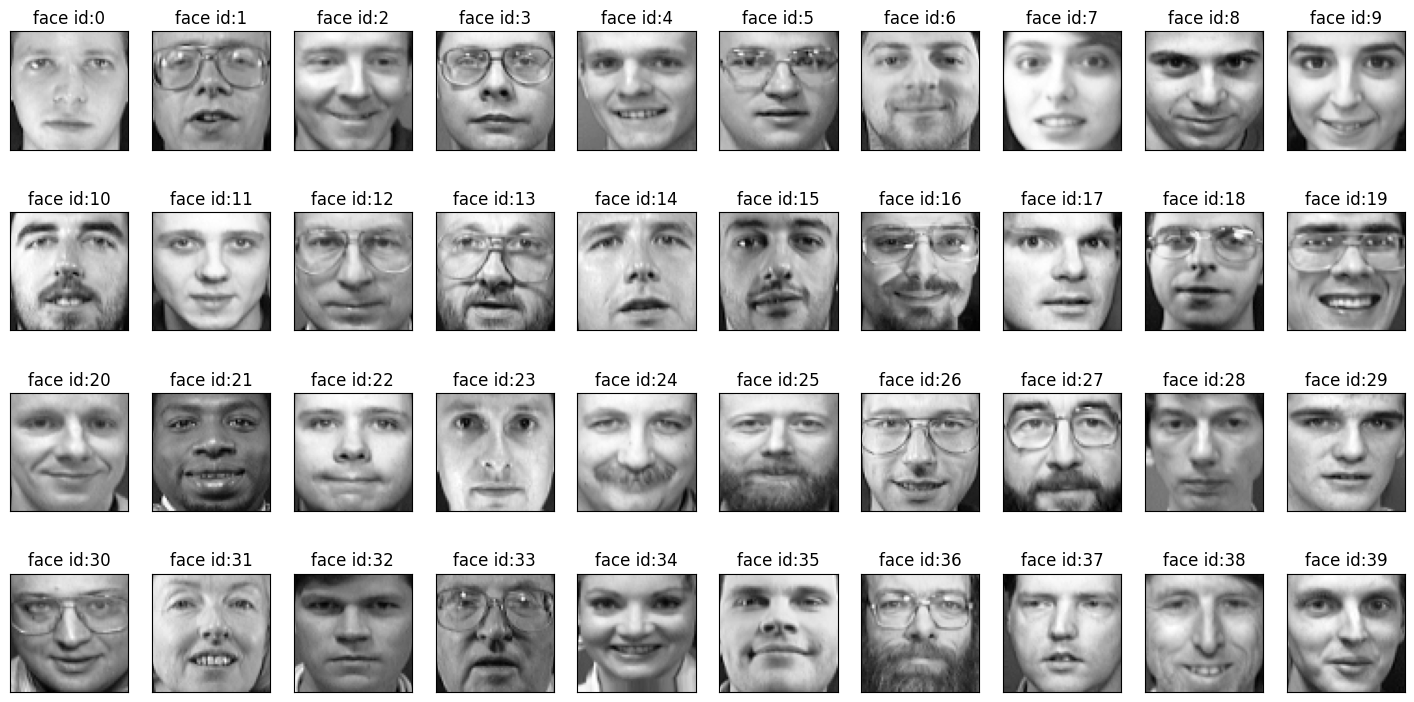
\includegraphics[width=0.5\textwidth]{images2/allimages.png}

\caption{\label{fig:Dataset Images} 
All persons in Olivetti Dataset}
\end{figure}


The collection, which consists of 400 face photos in total, has 10 unique photographs for each of the 40 participants\ref{fig:Dataset images by person}. The purposeful diversity of the Olivetti Dataset guarantees a comprehensive examination of facial expressions, lighting circumstances, and fine facial characteristics, rendering it a priceless resource for evaluating the resilience and versatility of face recognition algorithms. Given that the face photos were taken at various periods, the temporal aspect of the dataset gives it an additional realistic touch. Because of this temporal variance, researchers may assess the models in dynamic environments that replicate real-world situations in which people's appearances may change over time.
\begin{figure}[H]
\hspace*{-1.5cm}
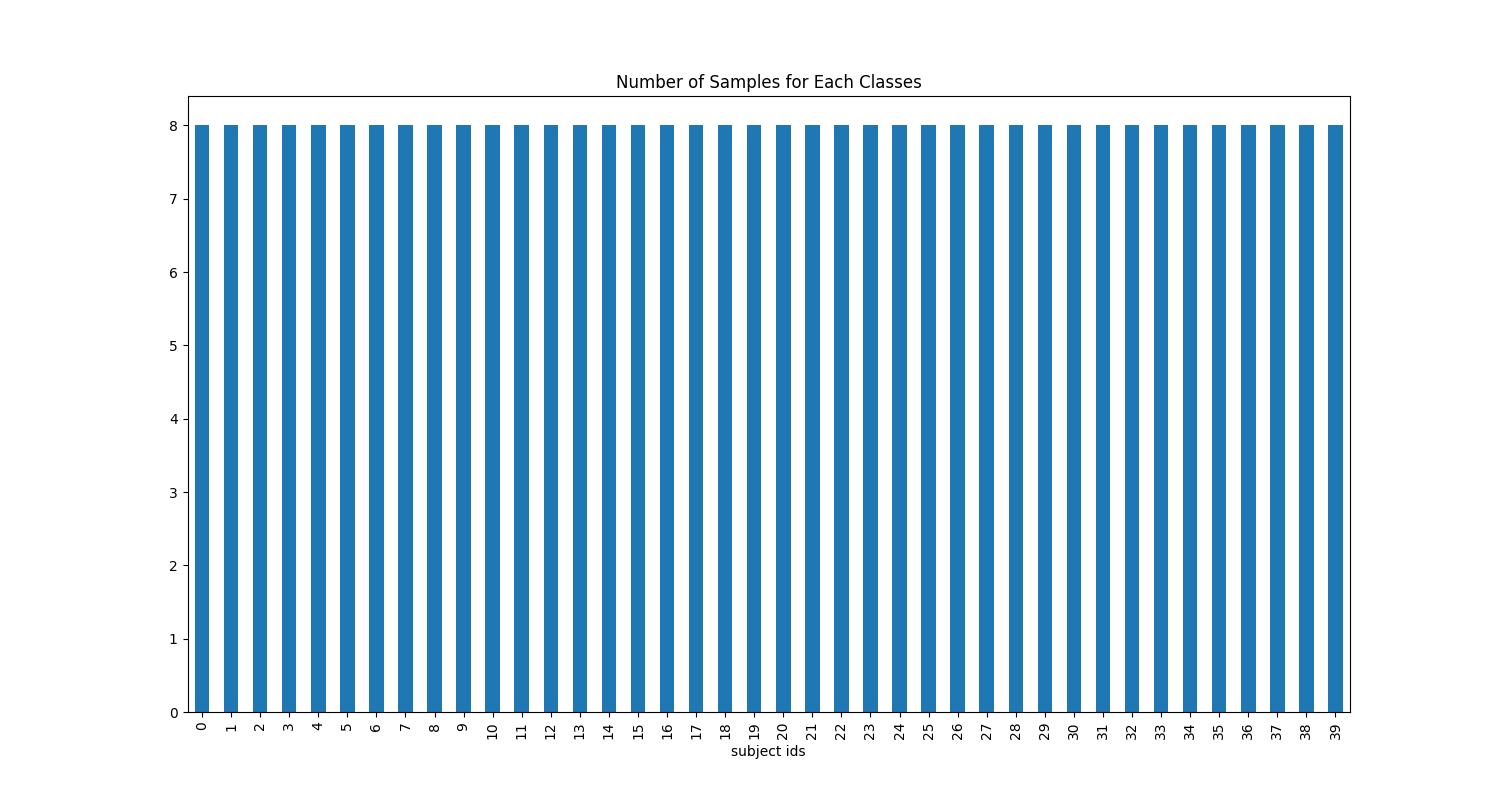
\includegraphics[width=0.6\textwidth]{images2/distribution.png}

\caption{\label{fig:Distribution of the Data} 
Data Distribution}
\end{figure}


\begin{figure}[H]
\centering
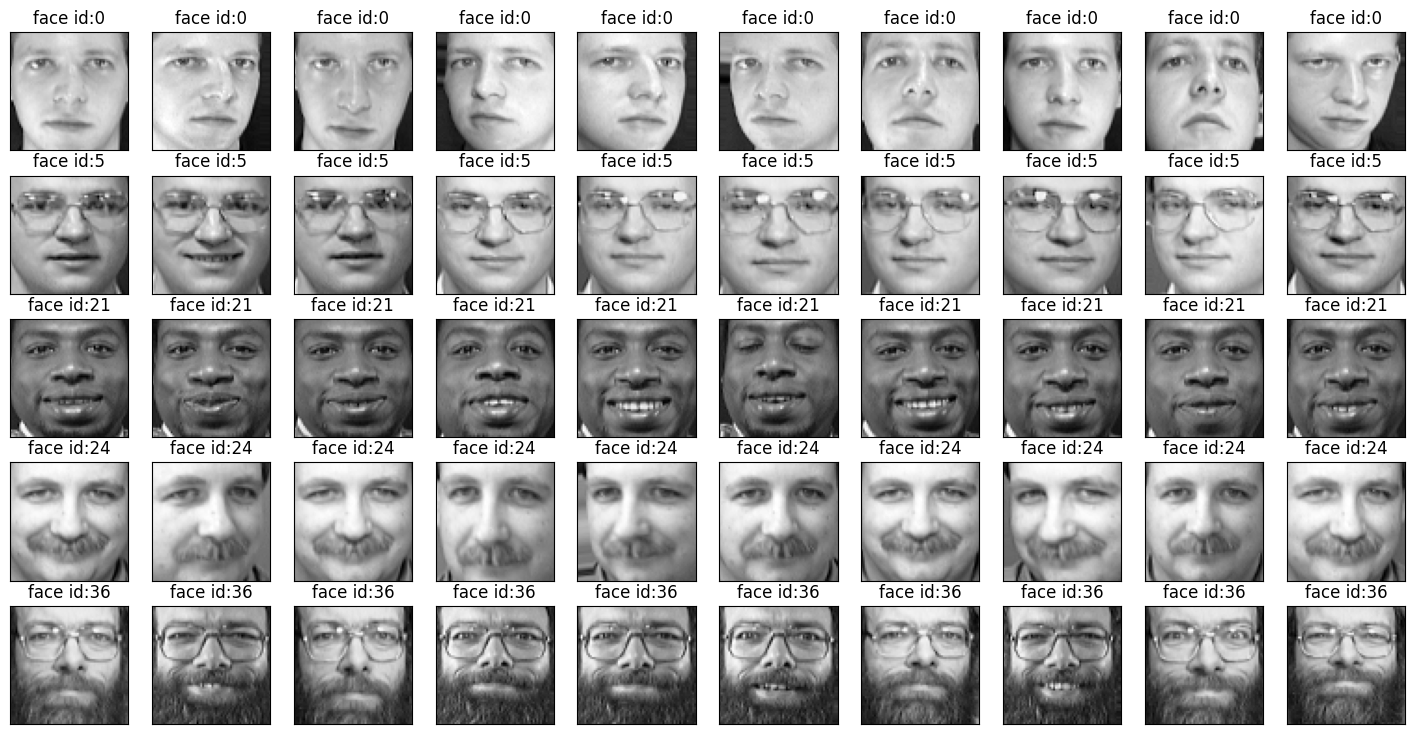
\includegraphics[width=0.5\textwidth]{images2/severalphotos.png}

\caption{\label{fig:Dataset images by person} 
Images by person}
\end{figure}



By treating picture characteristics consistently, uniformity is preserved. Every face image has a black backdrop, which reduces unnecessary visual components and draws attention to the important aspects of each face. With every image having the same size of 64 by 64 pixels, the grayscale format guarantees clarity and focus. Additionally, the pixel values have been scaled to the [0, 1] interval to enable uniform data representation and improve the dataset's suitability for use with a variety of machine learning models. In order to optimize the dataset for supervised learning tasks, the 40 individuals' names have been converted into integers between 0 and 39. Face recognition models can be trained and evaluated more effectively thanks to this encoding, which also makes the labeling process simpler. To conclude, the Olivetti Dataset is revealed as a dynamic collection that captures the essence of facial diversity over time, in addition to being a repository of facial images. This dataset provides a solid basis for researchers and practitioners looking to advance the field of face recognition through empirical analysis and model development, thanks to its careful preprocessing and thoughtful approach to image properties.

\section{State Of the Art}


In the realm of facial recognition, the state of the art continually evolves, driven by advances in machine learning and computer vision. Recent years have witnessed significant breakthroughs, propelled by the emergence of sophisticated models, increased computational power, and expansive datasets.
On Kaggle\cite{facerecognition} we found some results for this dataset\ref{fig:results} and our mission is to choose some machine learning models and improve the accuracy so that we can then compare some values and reach conclusions that can evolve this area of face recognition.
\begin{figure}[H]
\centering
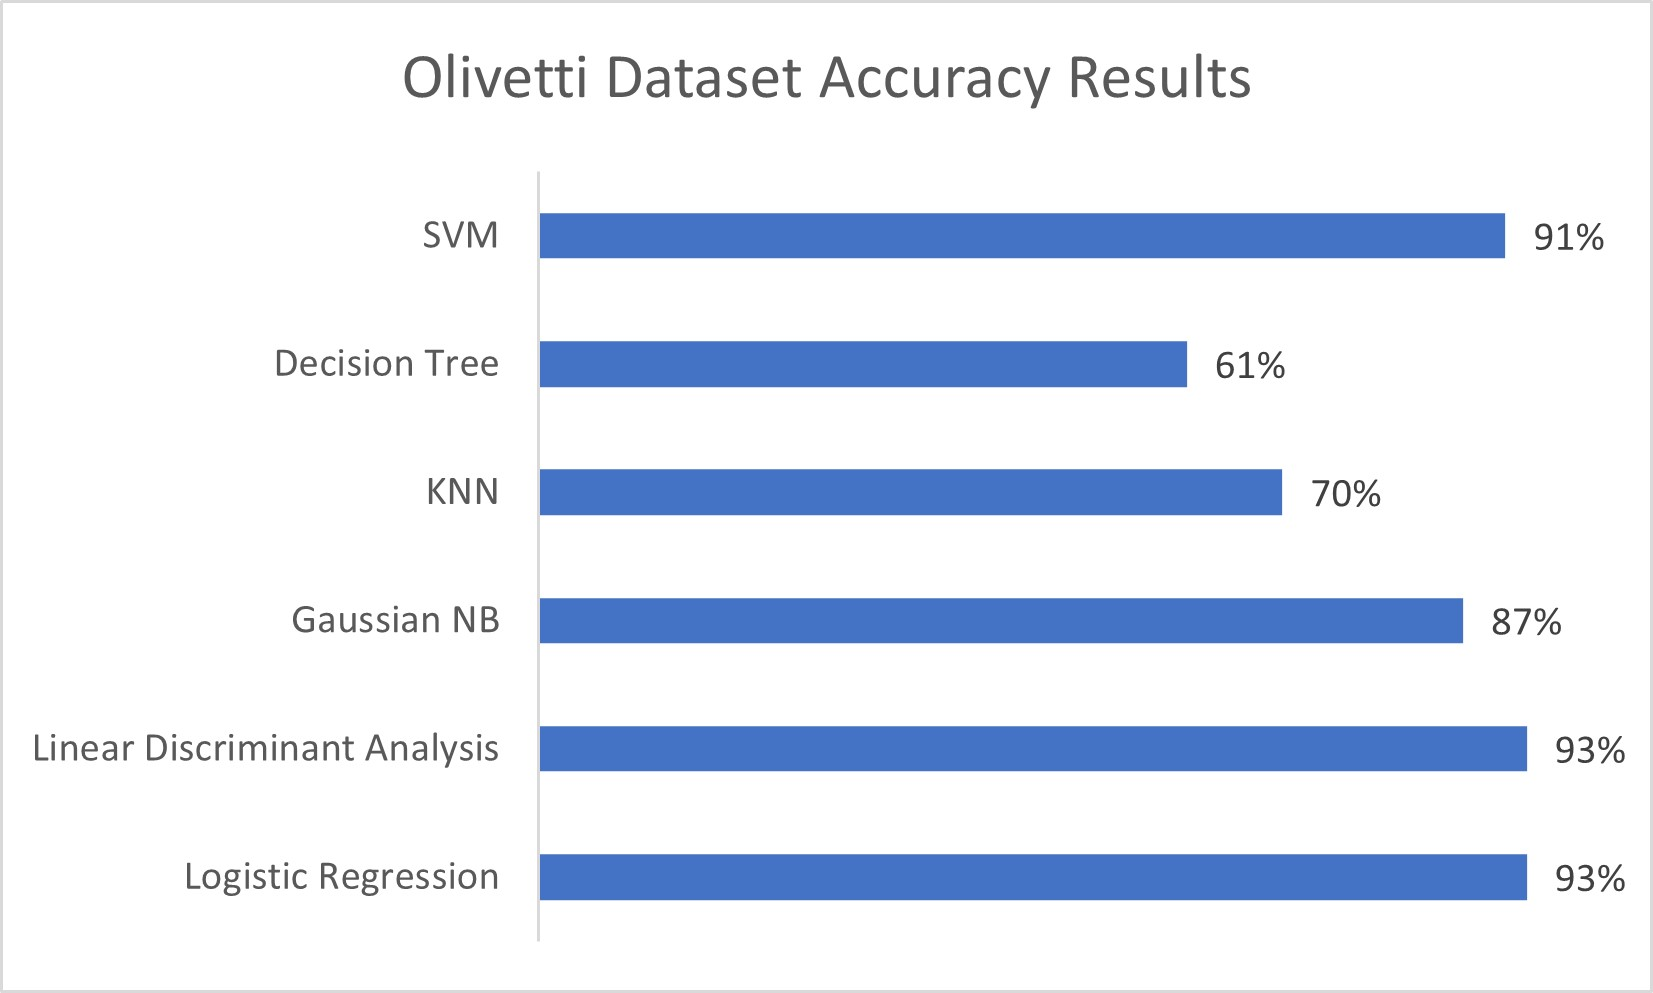
\includegraphics[width=0.5\textwidth]{images2/GraphicOD.jpg}
\caption{\label{fig:results} Examples Results of Olivetti Dataset}
\end{figure}

We read a few publications to provide us with a foundation for selecting the finest ones to create for facial recognition. SVMs have been effectively used for face recognition applications like face detection and face identification. They have demonstrated proficiency in managing intricate and diverse facial features\cite{paper5} \cite{paper2}.

\subsection{A novel fast hybrid face recognition approach using convolutional Kernel extreme learning machine with HOG feature extractor\cite{paperContext}}
Because of the advancements in machine learning techniques, the field of face recognition has grown rapidly. Remarkably, the development of machine learning algorithms—especially those based on deep learning—has improved facial recognition systems' accuracy and effectiveness significantly.
Historically, statistical models and manually created features have played a major role in face recognition systems. On the other hand, convolutional neural networks (CNNs) are now preferred in the field of face recognition due to the rise of deep learning. CNNs are particularly good at face recognition jobs because they can automatically identify complex patterns and characteristics from input data.
One of the most important benefits of using machine learning for face recognition is its ability to deal with variations in facial appearance, such as changes in lighting, position, and occlusions. Machine learning algorithms are able to learn to extract robust and distinguishable features from face photos, which enables more accurate detection in difficult situations.
Moreover, the utilization of machine learning methodologies has enabled the development of face recognition systems that are more efficient and expandable. Face recognition algorithms have become more realistic for real-world applications due to the reduction of processing needs with the implementation of techniques .

\subsection{Machine Learning Methods and Tools for Facial Recognition
Based on Multimodal Approach\cite{paper2}}
With strong algorithms at its core that can identify complex patterns in data, facial recognition represents a formidable frontier in machine learning. Support Vector Machines (SVM) stand out among these algorithms as a particularly effective tool for facial feature recognition and classification. SVM is particularly useful in the field of facial recognition, where it is used to train models that correctly identify and categorize people according to their facial features. Strategically classifying data points within a high-dimensional space is accomplished by SVM through the construction of a hyperplane. This procedure becomes particularly important in the context of facial recognition, where a labeled dataset of facial images, each closely associated with a unique person, is used to refine the algorithm.


\subsection{Face Recognition System Using Machine Learning Algorithm \cite{state1}}
\par The paper discusses the use of machine learning algorithms and principal component analysis (PCA) in a face recognition system. 


\par PCA is a feature extraction technique used to transform the original face images into a more compact and representative feature space. It reduces the dimensionality of the face images while preserving the most important information. 
By combining machine learning algorithms with PCA, the face recognition system can effectively handle variations in lighting, facial expressions, and partial occlusion enabling accurate and robust face recognition.
\par
The combination of the Viola Jones algorithm and Principal Component Analysis (PCA) is used for quick and accurate face detection.
Support Vector Machines (SVM) is considered a valuable classification method for face recognition due to its ability to generate reliable results. SVM constructs a hyperplane with the highest possible Euclidean distance to separate the nearest qualified instances
\par The paper, also includes algorithms like Naïve Bayes, Multilayer Perceptron, and Linear Discriminant Analysis. 
\par The highest accuracy achieved in the paper is 100\%, using the PCA+Linear Discriminant Analysis for configuration C and the second  is 97\% accuracy using PCA+Linear Discriminant Analysis approach for configuration B.
\subsection{Gabor Filter-Based Face Recognition Technique\cite{state2}}
\par The supervised facial recognition system proposed in the paper consists of three main components: 2D Gabor filter-based feature extraction, a supervised classifier, and a threshold-based verification technique.

The first step in the identification process is face feature extraction. The authors propose using 2D Gabor filters, which are widely used in image processing.
Gabor filters are band-pass linear filters that are defined by a harmonic function multiplied by a Gaussian function. They are used to extract features from facial images.
The authors choose to use symmetrical Gabor filters at various orientations, frequencies, and standard deviations to obtain a powerful 3D face feature vector.

After the feature extraction process, a supervised classifier is used for facial feature vector classification.
The classifier is based on minimum average distances and the squared Euclidean metric.
The goal of the classifier is to assign each feature vector to a specific face class, representing a registered user of the system.

In the verification stage, the system needs to decide whether an input image represents the face of a registered user.
The proposal is an automatic threshold-based verification approach, which consists in computation of a proper threshold value, considering the overall maximum distance between any two training face feature vectors corresponding to the same registered user.
The average distances from each face class are compared with the threshold value. If the average distance for an image from a class is greater than the threshold, the image is invalidated and rejected from the face class.

This technique achieves a high facial recognition rate, with approximately 90\% accuracy.  The performance parameters, Precision and Recall, have shown high values. The technique has been tested on hundreds of frontal face images, resulting in a high recognition rate, however, the recognition rate is lower for images representing rotated or non-frontal faces. 
\subsection{ Face Recognition with Very Deep Neural Networks \cite{state3}}
\par The authors of this paper chosen to use DeepID3, which is a very deep neural network architecture, designed for face recognition. It is built upon the stacked convolution and inception layers proposed in VGG net and GoogLeNet. The main idea behind DeepID3 is to leverage the learning capacity of very deep neural networks to improve the performance of face recognition.

\par There are two versions of DeepID3: DeepID3 net1 and DeepID3 net2. DeepID3 net1 consists of multiple convolutional layers followed by pooling layers. It also includes additional fully-connected layers branched out from intermediate layers, which helps to learn better mid-level features and makes optimization of the network easier. The top layers of DeepID3 net1 are replaced by locally connected layers, which allows them to form more expressive features with a reduced feature dimension.

DeepID3 net2 follows a similar structure as DeepID3 net1, but it uses inception layers in later feature extraction stages. Inception layers are a type of convolutional layer that includes multiple parallel convolutional operations with different filter sizes. This helps to capture features with larger receptive fields .

\par Both DeepID3 net1 and DeepID3 net2 include joint face identification-verification.
The joint identification-verification supervisory signals are added on fully connected layers following each pooling layer. This means that the network is trained not only to classify faces into different identities but also to verify whether two face images belong to the same person or not. By incorporating both identification and verification tasks, the network can learn more discriminative and robust features for face recognition.

Compared to other neural network architectures used in face recognition:
\begin{itemize}
    \item DeepID3 networks are significantly deeper. DeepID3 net1 has ten to fifteen non-linear feature extraction layers, while DeepID3 net2 has even more layers. 
    \item DeepID3 networks, use unshared neural weights in the last few feature extraction layers. 
    \item DeepID3 networks add joint identification-verification supervisory signals to early layers.
    \item DeepID3 net2 incorporates inception layers in later feature extraction stages
\end{itemize}

The DeepID3 architectures achieved impressive results . The ensemble of the two architectures (DeepID3 net1, DeepID3 net2), achieved a face verification accuracy of 99.53\% on the LFW dataset.


\section{Methods}
\subsection{K-Fold Cross Validation}
\par To verify our model's performance it is mandatory to do some kind of validation, the one we think is more reliable is K-Fold Cross Validation. This validation consists on splitting the data in two sets, the train set, that will be used for training the model and update the parameters,the validation set is the remaining data that will be used to observe the performance of the model through data validation.It's important guarantee  data balancing after splitting data  to avoid biased results. 
This process will be repeated k times, in our case k = 4 (so, 20\% validation data and 60 \% train data ) and in every iteration, the train and validation sets will be chosen  with fixed size and fixed examples,i.e, the validation set won't have the same examples in each fold. Also, it is important to reference that every fold iteration isn't independent, this is because the final weight parameters (theta) of every iteration are used as initial theta of the next one. This process is called fine tunning.
Besides this, we still have a test set, which is a set that will never be used for learning purposes, only for validation, and it will take the remaining data, that corresponds to 20 \%.

\subsection{Confusion Matrix}
\par To validate our results we will use a confusion matrix. The confusion matrix give information of the true positives, false positives, true negatives and false negatives  obtained from the learning process. How do we get that information? We will obtain a list with length n as output of the model, being n the number of labels, and every element of the list will have a number between 0 and 1 corresponding to the probability of the prediction being the actual class. We will consider the prediction, the class with the highest probability.
At the end, since the data is balanced, we will only measure the performance of the model with accuracy metric.
\subsection{Roc Curve and AUC}
\par To validate our model's final performance, we will use some metrics that serves that purpose, AUC and Roc Curve, besides that, they will be used to compare models, ours and other ones from different scientific papers.
\par ROC curve demonstrates how well a test can distinguish between true positives and false positives, it aids in evaluating the trade-off between sensitivity and specificity.
\par The Area Under the Curve, or AUC is a number between 0 and 1 that indicates the area under the ROC curve. When the test can totally distinguish between the two groups, it is said to have perfect discrimination (AUC of 1). An AUC of 0.5 suggests that the test has no discriminatory ability.
\subsection{Coding}
\par This project was developed in Python programming language alongside with many libraries of it. We Will enumerate them and briefly describe for what they were used.
\begin{itemize}
  \item tensorflow.keras -Build the neural network.
  \item sklearn.model\_selection \cite{sklearn} - Split the data and K-Fold Validation
  \item sklearn.metrics - Confusion matrix, Accuracy Score and roc curve
  \item sklearn.discriminant\_analysis - Discriminant Analysis
  \item sklearn.decomposition - PCA
  \item pandas \& numpy - Data management
  \item sklearn.preprocessing - Data Normalization
  \item scipy.stats - Features Correlations
  \item matplotlib.pyplot - Data visualization
\end{itemize}
\subsection{Description of the Machine Learning Algorithms}
\subsubsection{Principal Component Analysis}
\par Principal Component Analysis (PCA) is a widely used technique in various fields such as image processing, signal processing, feature extraction, and data compression. The main goal of PCA is to transform the original high-dimensional data into a new set of uncorrelated variables called principal components. PCA relies on the covariance matrix of the data. The principal components are the eigenvectors of this covariance matrix, and the corresponding eigenvalues represent the amount of variance explained by each component.

These components capture the maximum variance in the data, allowing for a more concise representation. The first PC (PC1) is chosen to maximize the variance and the following components follow the same pattern with the remain data until n = (number of features) in PCn, the programmer choose the more convenient number of PCs for the problem to be solved.

\begin{figure}[H]
\centering
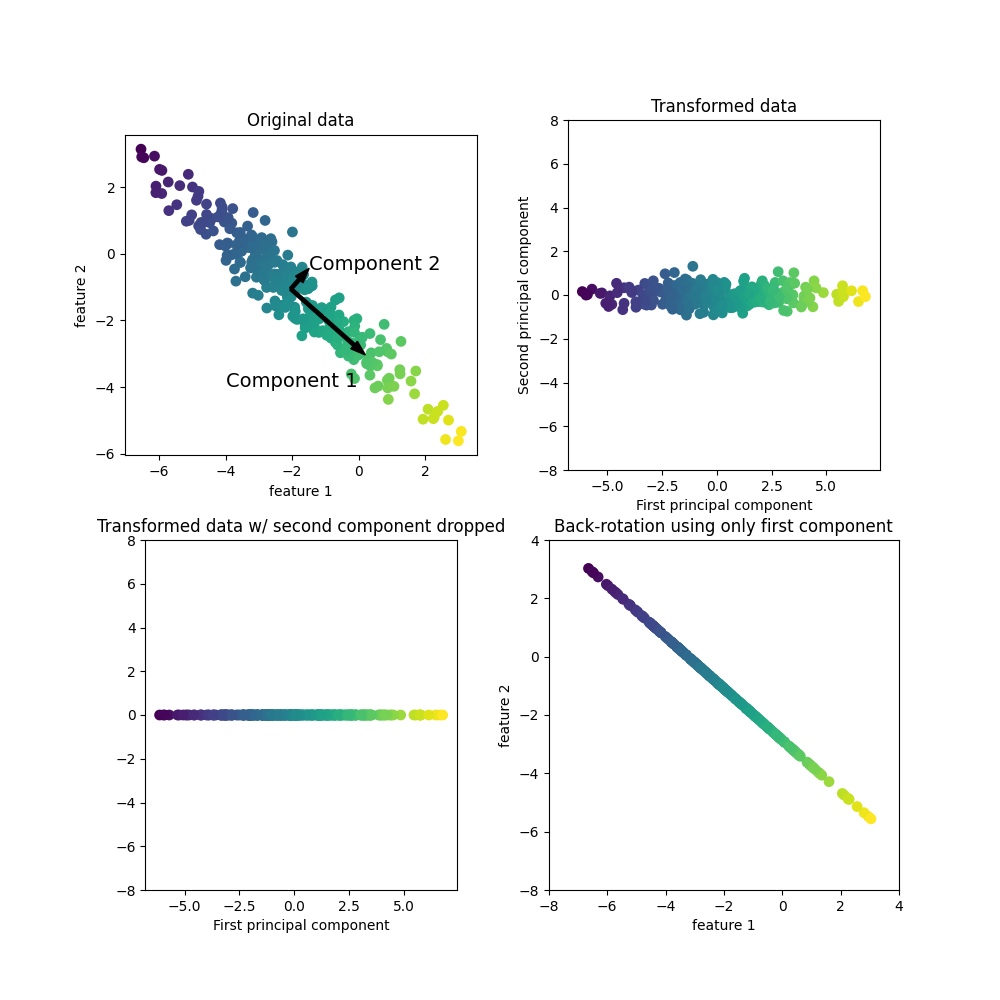
\includegraphics[width=0.5\textwidth]{images2/pca.png}
\caption{\label{fig: pca} PCA demonstration}
\end{figure}
\par The scenario above \ref{fig: pca}  demonstrates a straightforward example using a synthetic two-dimensional dataset. In the initial visualization, data points are color-coded to distinguish between them. The algorithm's first step involves identifying the direction of maximum variance, denoted as "Component 1." This direction represents the axis along which the data exhibits the most significant variability .
Subsequently, the algorithm seeks an orthogonal direction  to the first one. In the context of two dimensions, there is only one possible orientation at a right angle. However, in higher-dimensional spaces, there exist numerous orthogonal directions (infinite possibilities) to explore. 
\cite{pca}
\subsubsection{Linear Discriminant Analysis}
\par Like PCA, Linear Discriminant Analysis is a technique to reduce data dimensionality,
LDA aims to find an orientation, represented by the vector W, that transforms high-dimensional feature vectors belonging to different classes into a lower-dimensional feature space.
The goal is to ensure that the projected feature vectors of each class in this lower-dimensional space are well-separated from those of other classes.
\par  In this figure \ref{fig: lda}, two-dimensional feature vectors are reduced to a one-dimensional feature vector.
Three classes, denoted as C1,C2 and C3, have feature vectors. The objective is to find an orientation (W) such that the projected feature vectors on a line are maximally separated by class.

The orientation $\vec{W}$ does not provide good separation, but by rotating the line to orientation W the projected feature vectors become well-separated from those of other classes.
The conclusion is that W is a better selection than $\vec{W}$.
The value of W is obtained by maximizing the Fisher’s criterion function J(W).
This function depends on three factors: the orientation W the within-class scatter matrix (SW), and the between-class scatter matrix (SB).
If the dimensionality reduction is from a d-dimensional space to an h-dimensional space, then the size of the orientation matrix W is determined accordingly.
\begin{figure}[H]
\centering
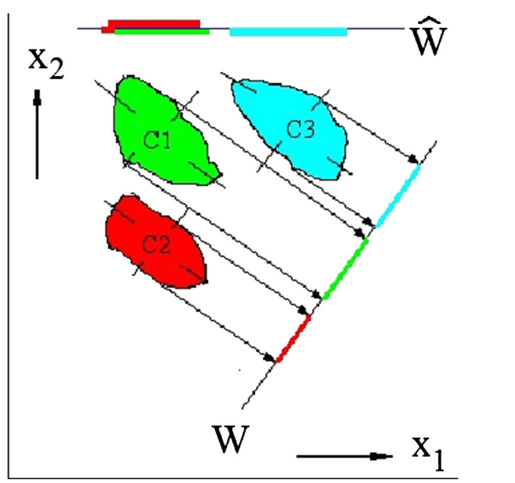
\includegraphics[width=0.4\textwidth]{images2/lda.png}
\caption{\label{fig: lda} LDA demonstration}
\end{figure}
Image taken from \cite{lda}

\paragraph{Decision Rule in LDA}

Once the Linear Discriminant Analysis (LDA) model has been trained on the data, it needs a rule to assign new, unseen data points to one of the classes. This decision-making process involves calculating probabilities and choosing the class with the highest probability for each data point.

The decision rule in LDA is typically based on Bayes' Theorem and the assumption of normally distributed data within each class. The decision rule involves calculating the posterior probabilities of each class given a new data point and assigning the data point to the class with the highest posterior probability.

The Bayes' Theorem formula for a binary classification problem (two classes) is as follows:

\[
P(C_k | x) = \frac{P(x | C_k) \cdot P(C_k)}{P(x)}
\]
\begin{itemize}
    \item \( P(C_k | x) \) is the posterior probability of class \( C_k \) given the data point \( x \).
    \item \( P(x | C_k) \) is the likelihood of the data point \( x \) given class \( C_k \).
    \item \( P(C_k) \) is the prior probability of class \( C_k \).
    \item \( P(x) \) is the probability of the data point \( x \).
\end{itemize}

The decision rule is then applied by choosing the class with the highest posterior probability. In a binary classification scenario, if \( P(C_1 | x) > P(C_2 | x) \), the data point is assigned to class \( C_1 \).
\cite{scikit-learn}
\subsubsection{Artificial Neural Network}
\par Neural network is a machine learning model in-
spired by the structure of the human brain. They
are composed by interconnected nodes divided
by layers. Those layers are input layer, hid-
den layer and output layer. The nodes are ob-
tain through a combination of the previous layer
nodes, except the input layer, and they are trans-
formed by the activation function.
The learning process is the adjustment in the
weight of each feature in order to achieve the
maximum performance of the model, in this
case, each node. This model, specifically, uses
one method called Backpropagation, where the
output layer propagates the error through all
layers until it reaches the input layer .

\subsubsection{Logistic Regression}
Logistic regression\ref{fig:cost_func} is a useful and comprehensible tool for binary classification tasks in the field of face recognition. Although logistic regression has its roots in linear regression, its use in determining whether a face image belongs to a particular person fits in well with the problem's inherent dichotomy. We use the Olivetti Dataset to investigate logistic regression in the context of face recognition. Logistic regression emphasizes transparency in model decisions and is a popular choice for real-world scenarios due to its interpretability and simplicity. We hope to advance the state-of-the-art by advancing practical implementation of our understanding of logistic regression in face recognition.
\begin{figure}[H]
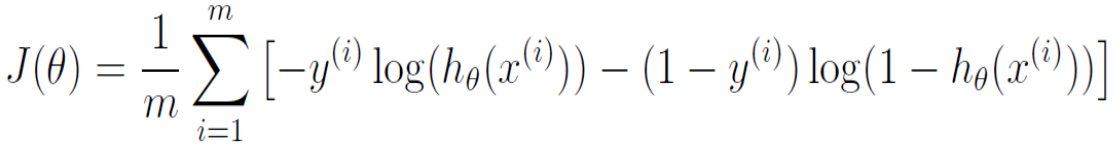
\includegraphics[width=0.5\textwidth]{images2/Screenshot from 2023-11-05 21-14-53.png}
\centering
\caption{\label{fig:cost_func} Logistic Cost Function}
\end{figure}

\subsubsection{Suport Vector Machine}
Support Vector Machine (SVM) is shown to be a reliable and efficient algorithm. One well-known supervised machine learning model that excels at classification tasks is SVM. SVM functions in the field of facial recognition by determining the ideal hyperplane for separating various facial features, allowing the development of a highly discriminative model. SVM is particularly good at identifying complex patterns and minute variations that are necessary for precise face identification when working with the Olivetti dataset, which is a collection of facial images. SVM excels at handling high-dimensional data and identifying intricate relationships, which makes it especially well-suited for the complex task of facial recognition. When it comes to face recognition, the SVM algorithm aims to maximize the margin between various face classes so that people can be distinguished from one another. SVM can implicitly map data into higher-dimensional spaces using kernel functions, which improves its ability to capture complex facial features. SVM's adaptability and strong face generalization to new faces become important advantages as we use the Olivetti dataset to leverage it for face recognition. SVM is a useful tool for obtaining accurate and dependable face recognition results because of its robustness and refined capacity to handle complex facial features.


\subsection{Pipeline architecture}

\par The figure \ref{fig: arch} demonstrates an overview of the pipeline of our model. We start by loading the data, that is already normalized, all values belong to the interval [0,1].
The following list describes all the approaches taken in the work, who is in tune with the figure's information. 
\begin{itemize}
  \item PCA + LDA
  \item LDA
  \item LR
  \item SVM
  \item PCA + LDA + NN

\end{itemize}

\begin{figure}[H]
\hspace*{-0.5cm}
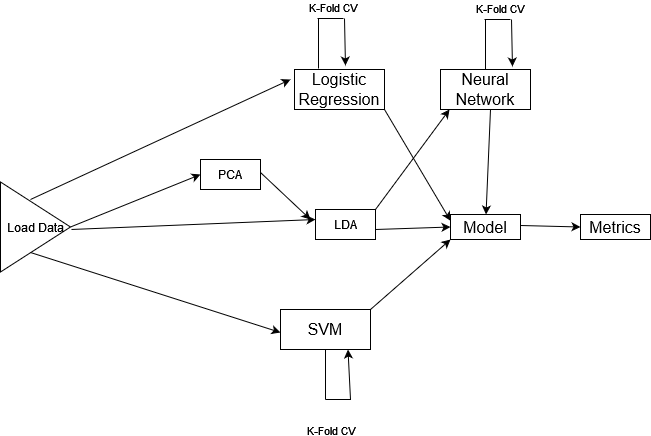
\includegraphics[width=0.5\textwidth]{images2/arch.png}
\caption{\label{fig: arch} Pipeline architecture}
\end{figure}
Note that NN is only viable when combining with PCA + LDA, because the usage of raw data with this model implies a huge amount of parameters, turning to be a really slow and heavy machine learning model.
\subsection{Training ML Algorithm}
\subsubsection{Principal Component Analysis}
\par In this work, PCA was used to reduce the number of features, increasing the speed  of the model training, and hopefully, increase the performance of the model.
\par This figure \ref{fig: pca2} represents the data for 10 different people over two different components, and, we can notice that the classes aren't separated in the space, however, the data is well represent in a lower dimension.
\begin{figure}[H]
\centering
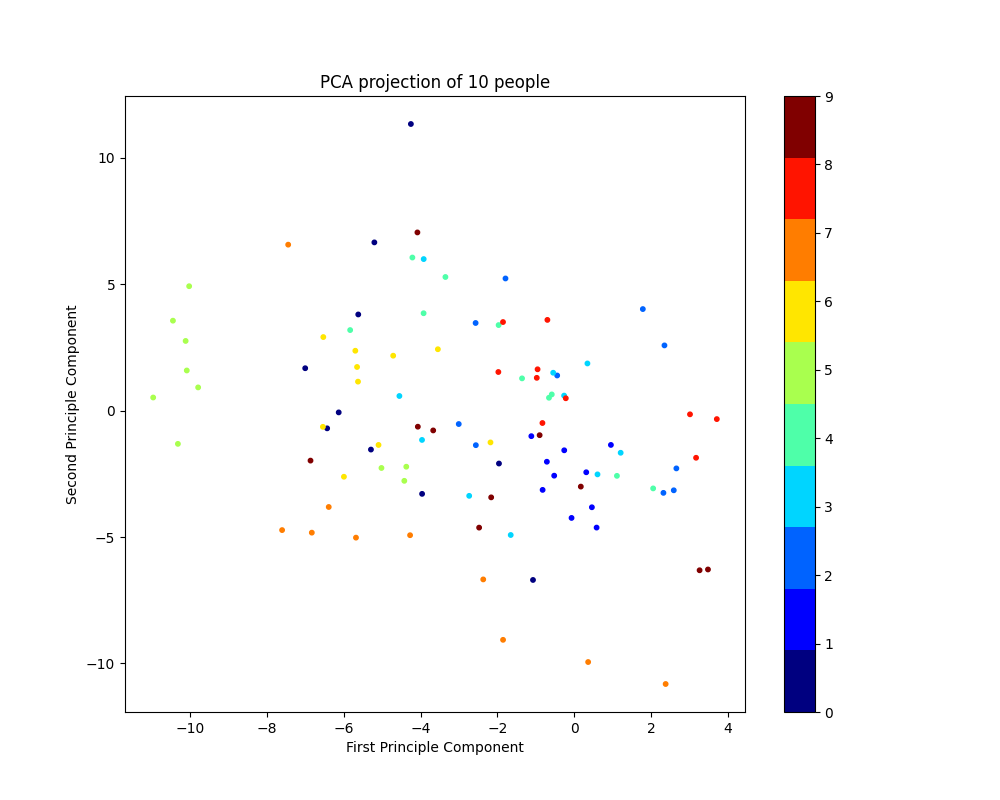
\includegraphics[width=0.6\textwidth]{images2/pca2.png}
\caption{\label{fig: pca2} Data represented by two principal components}
\end{figure}
Our goal is to find the minimum number of components that are capable of representing the data without lost of information, lose as least as possible. The figure \ref{fig: pca3} represents the explain variance of the principal components, i.e., the variability of data . As we can see, variance stabilises more or less since 90 components,so we are using 90 principal components in our model. 
\par  We can visualize the principal components by reshaping each of them into a 64 × 64 matrix that corresponds to the pixels in the original dataset. 
The figure below\ref{fig: eigen} displays the first 10 principal components.

\begin{figure}[H]

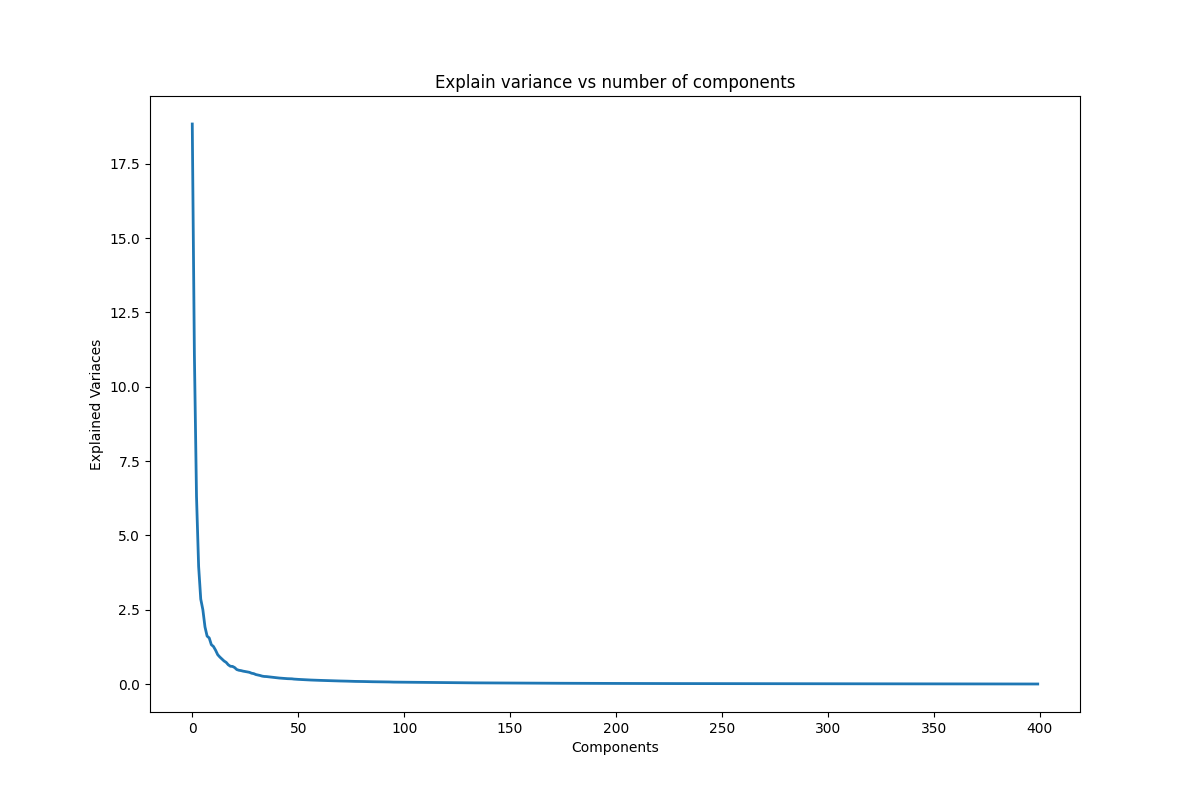
\includegraphics[width=0.5\textwidth]{images2/pca3(3).png}
\caption{\label{fig: pca3} Explain variance vs number of components}
\end{figure}

\begin{figure}[H]
\centering
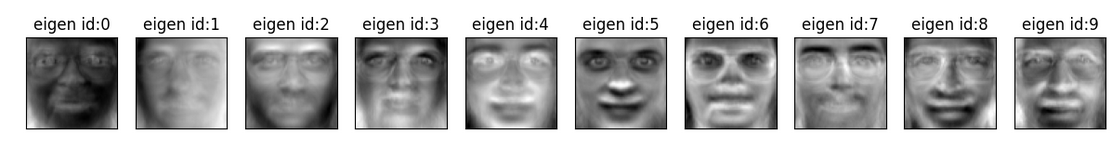
\includegraphics[width=0.5\textwidth]{images2/eigen.PNG}
\caption{\label{fig: eigen} Eigen Faces}
\end{figure}


\subsubsection{LDA}
\par Lda will have 3 approaches:
\begin{itemize}
    \item Classifier using original data
    \item Classifier using PCA as input
    \item Feature extraction
\end{itemize}
\par All the options above include a first step of feature extraction, however the number of components vary, because, when the LDA is used as input of another model, a grid search must be made together with that model.
\par To  maximize the performance, a grid search will be done with a 4-fold cross validation and the hyper-parameters considered will be shrinkage, number of components and solver.\break
The solver parameter specifies the algorithm to use when calculating the covariance matrix and can be svd,lsqr or eigen:

\begin{itemize}
    \item  svd - Uses the Singular Value Decomposition technique to compute the covariance matrix. It is suitable for both small and large datasets but is particularly efficient when the number of features is less than the number of samples.\footnote{svd isn't compatible with shrinkage}
    \footnote{The only solver compatible to be used as input in other models}
    \item lsqr - Based on the least-squares solution and is suitable when the number of features is greater than the number of samples. It is particularly useful for high-dimensional data.
    \item eigen - Based on the eigenvalue decomposition of the covariance matrix. It is suitable for small to medium-sized datasets.
\end{itemize}

\par Shrinkage is a regularization technique used in LDA to stabilize the estimation of the covariance matrix, especially when dealing with small sample sizes or high-dimensional data.
\break

\par As we can see in the figures \ref{fig: lda_grid} \ref{fig: lda_grid2} the best hyper-parameters for using original data and PCA are solver = svd/lsqr \& shrinkage = None and solver = svd/lsqr \& shrinkage = 0.1 (None if used with svd) respectively . In these two cases the number of components was not tuned, just later on, when combining with other models, because it doesn't influence in the lda algorithm's performance, so the least number of components was chosen, i.e., 1 component .

\begin{figure}[H]
\centering
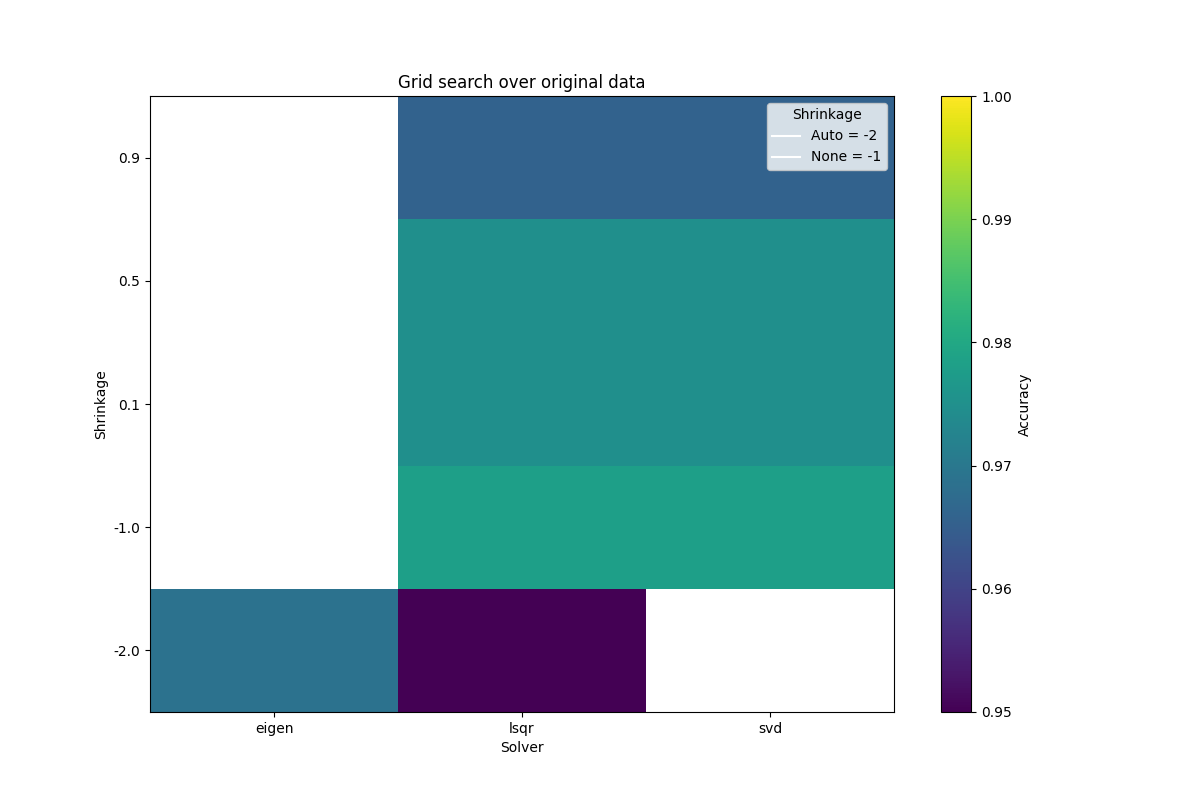
\includegraphics[width=0.6\textwidth]{images2/grid_lda1.png}
\caption{\label{fig: lda_grid} Grid search on LDA with original data as input}
\end{figure}

\begin{figure}[H]
\centering
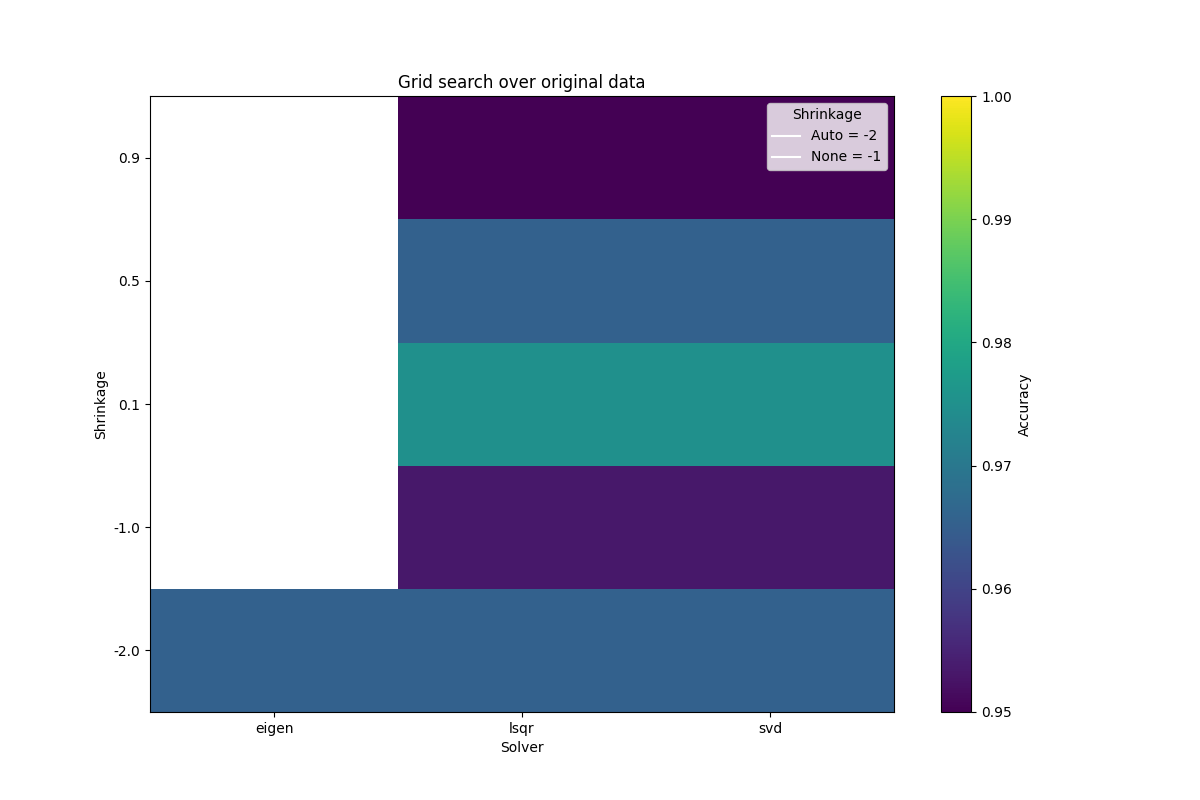
\includegraphics[width=0.6\textwidth]{images2/grid_lda_pca.png}
\caption{\label{fig: lda_grid2} Grid search on LDA with PCA as input}
\end{figure}
 \par If we observe the plot of the LDA components
 \ref{fig: lda_plot} we can clearly see a difference compared with PCA, the the points of each label have very low distance with each other, there is a clear tendency of forming groups with points of the same class. 

\begin{figure}[H]
\centering
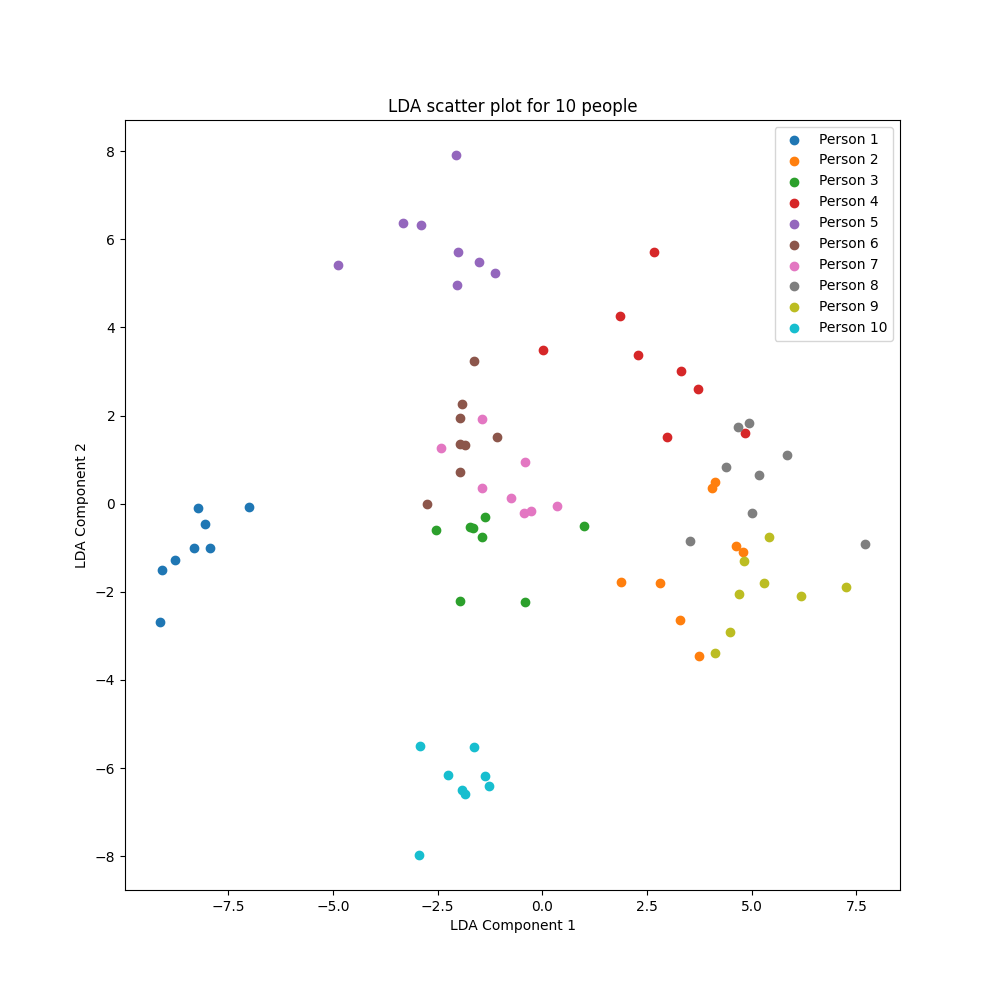
\includegraphics[width=0.5\textwidth]{images2/lda_plot.png}
\caption{\label{fig: lda_plot} Plot of LDA components for 10 people using PCA data as input}
\end{figure}

\paragraph{Results}
\par We can observe impressive results looking at \ref{fig:results_final_lda} and \ref{tab:lda_results}. The accuracy was really high, even with data that was unseen during training. We can have an higher impression of the model's performance observing the confusing matrix of test data, we can notice that the model only failed one prediction,, which is really good, predicting face id 39 instead of face id 4.
The results apply for LDA using original data and data from PCA, because they were identical.
\begin{table}[h!]
    \centering
\begin{tabular}{lrrr}
\toprule
{} &       accuracy  \\
\midrule
test  &  0.99 \\
train &  1.00  \\
val   &  0.98  \\
\bottomrule
\end{tabular}
    \caption{LDA Results}
    \label{tab:lda_results}
\end{table}



\begin{figure}[H]
\hspace*{-0.5cm}
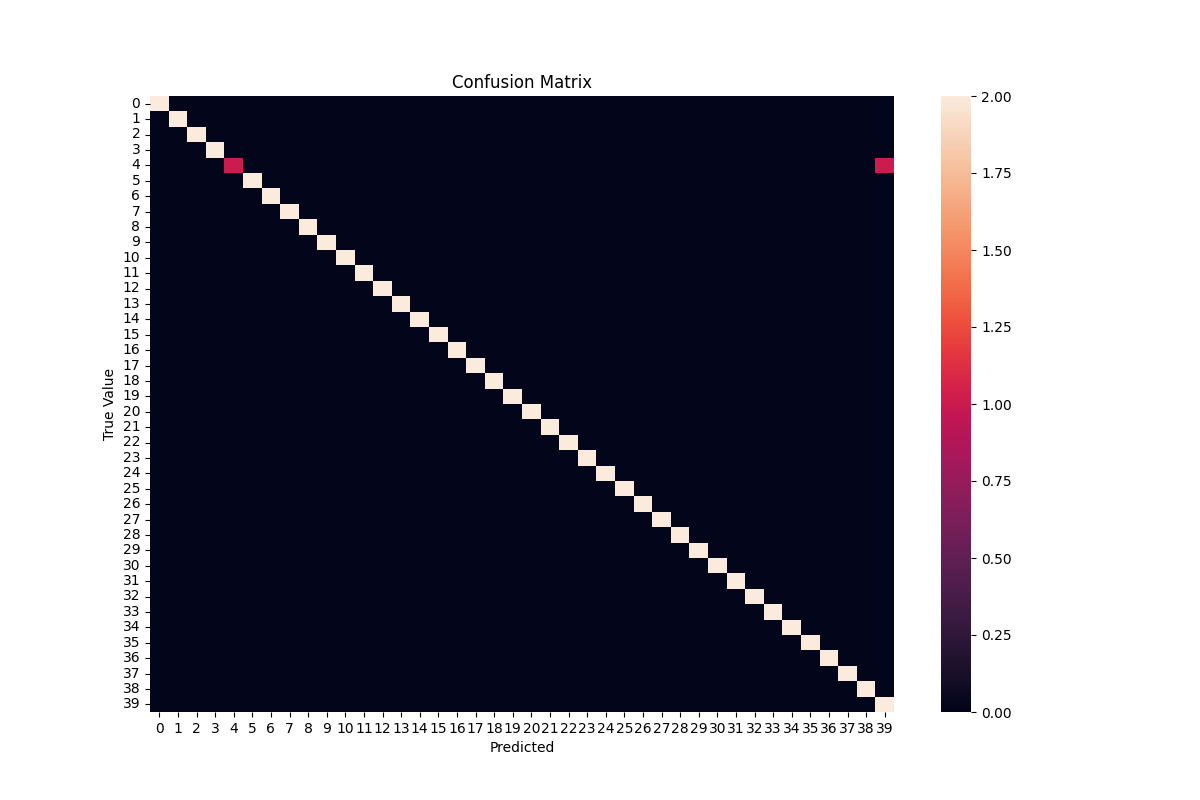
\includegraphics[width=0.6\textwidth]{images2/final_nn.png}
\centering
\caption{\label{fig:results_final_lda} LDA Confusion Matrix }
\end{figure}

\cite{scikit-learn}
\subsubsection{Neural Network}

\paragraph{Initial Configuration}
 \par Now that we know the basis about Neural Networks, it's time to present  the implementation.
 Our Neural network will use for its input, data from LDA algorithm, and LDA used data from PCA. The combination of these feature reduction techniques, allow us to use Neural Networks. Imagine that original data is used in NN, the images  are 64x64, so we have 4096 features as input, adding a 20 neurons hidden layer, for example, we will have a matrix  20x4097 containing all weight parameters meaning  81920 parameters, which is too heavy to compute.
\par Our Neural network is composed by n input neurons, which corresponds to the number of lda components (this value will be optimized later on), 30 neurons in the only hidden layer of the network and 40 in output that represents the 40 classes  in question, corresponding to the 40 different people. Two activation functions will be used, leaky relu(input layer) and sigmoid(hidden layer), both are very popular in classification problems. 
 \par The process of learning in conquered due to a cost function, the one chosen is categorical cross entropy loss function . This is a loss function used in multi-class classification problems. It measures the difference between predicted and actual class distributions, encouraging the model to output probabilities that align with the true labels. It requires one-hot encoding for target labels which requires transformation of labels to numeric, if they are not, and transform that  to ones and zeros, for example class 3 turns into [0 0 0 1] and class 0 to [1 0 0 0], taking into account 3 labels in this hypothetical scenario.
 Finally, adam was used as optimizer . It adapts learning rates for each parameter individually, incorporates momentum to accelerate optimization,i.e., guarantee that the loss function converges increasing the learning rate when the model is far from the convergence point and decrease learning rate in the opposite scenario.\par The figure \ref{fig:cost_func} shows the cost function, and we can notice that it converges and the cost value is stabilized, so the number of epochs is enough the get the best performance , which is 150.





\begin{figure}[H]

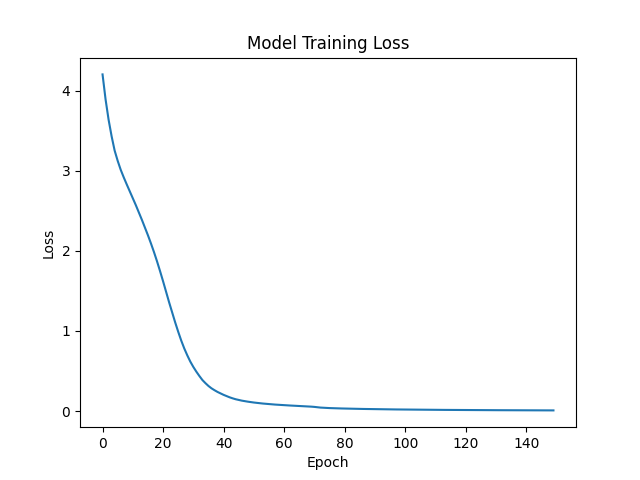
\includegraphics[width=0.5\textwidth]{images2/loss.png}
\centering
\caption{\label{fig:cost_func} Cost Function}
\end{figure}


\paragraph{LDA - Number of components}
\par It's important to decide the number of features used in the Neural Network. The best case possible would be 1 components because the learning process would be very fast, however, it may not be  enough data for the neural network learning.
\par Analysing the figure \ref{fig:lda_nn}, we can notice a stabilization of the accuracy since 10 components,so , 12 components will be used, to be sure.
\begin{figure}[H]
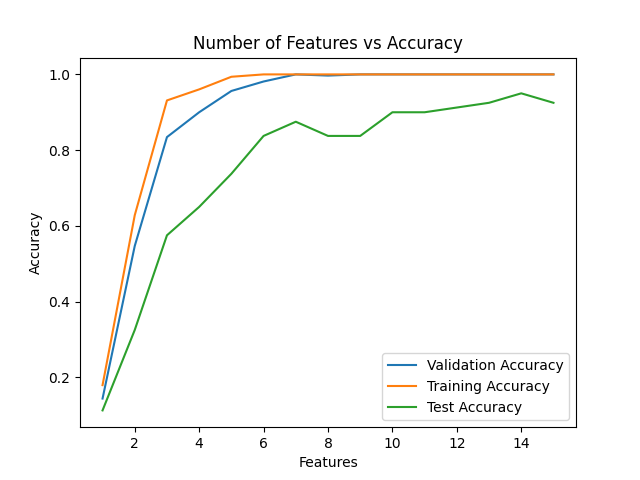
\includegraphics[width=0.5\textwidth]{images2/lda_nn.png}
\centering
\caption{\label{fig:lda_nn} Number of components vs Accuracy}
\end{figure}
\paragraph{Batch Size}
\par The batch size is a hyperparameter that determines the number of samples processed in each iteration during training.
Larger batch sizes can lead to better computational efficiency, allow parallel processing, which can speed up training, however,
smaller batch sizes introduce more randomness into the training process, potentially helping the model generalize better so,
It's essential to experiment with different batch sizes and evaluate the best value for our data-set. 
\par The figure \ref{fig:batch} describes that study, and we can notice that batch size doesn't influence the model performance except in the lower values, so the biggest value of batch size will be chose, which is 128, in order to improve training times.
\begin{figure}[H]
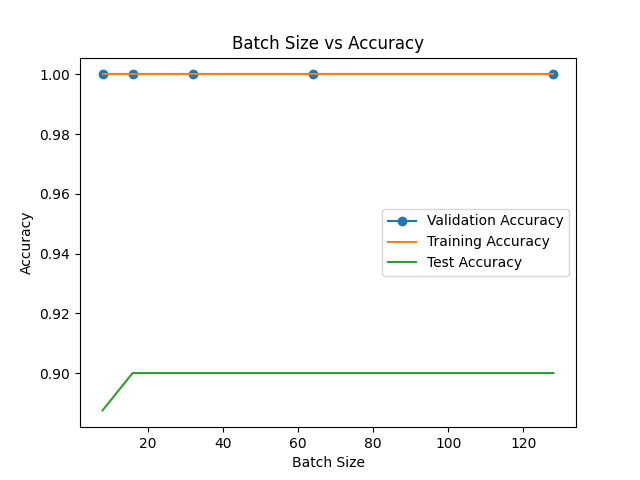
\includegraphics[width=0.5\textwidth]{images2/batch.png}
\centering
\caption{\label{fig:batch} Batch size vs Accuracy}
\end{figure}

\paragraph{Regularization}
\par The next hyper-parameter tuned in this model is lambda.The lambda will make all learning parameters (theta) more similar, in other words, the lambda will avoid an huge contribution of one feature to model, and a tiny contribution of another feature to the model, if that happens, the model will be closed on the training examples and will be more difficult predict unknown data, what's called overfitting.
\par We will only considered l2 regularization because l1 apply feature selection in some cases, and that is not desirable due to the feature reduction done previously by  by PCA and LDA . In this case, we tried various values of lambda between 0 (0 included, meaning non utilization of regularization) and 10. As we can see in \ref{fig:l2} The point where both validation and accuracy accuracy were high was at 0.1 
\begin{figure}[H]
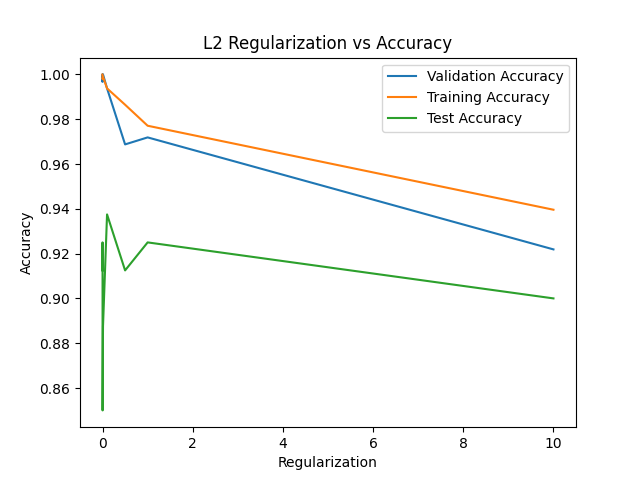
\includegraphics[width=0.5\textwidth]{images2/reg.png}
\centering
\caption{\label{fig:l2} L2 regularization vs Accuracy}
\end{figure}
\paragraph{Hidden Layer}
\par Another one of the hyper parameters that we can tune in order to increase the performance of the algorithm  is the number of neurons in the hidden layer. The best way to find the value that maximizes the performance  is through data visualization, so, analyzing the results obtain in the figure \ref{fig:neurons}, we note the better results in both test and validation data when using 30 neurons in the hidden layer.


\begin{figure}[H]
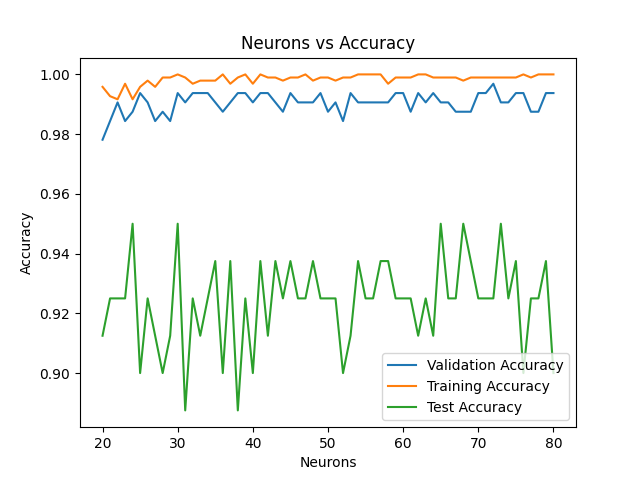
\includegraphics[width=0.5\textwidth]{images2/neurons(1).png}
\centering
\caption{\label{fig:neurons} Accuracy vs Neurons}
\end{figure}

\paragraph{Activation functions}
\par The last hyper parameter to optimize is the activation, something with impact in the model's performance, they are responsible to transform the output of one layer as an input of another layer. For the realization of this experiment, the most popular activation functions,as we can see in the figure \ref{fig:activation} . Note that the first activation function belongs to the hidden layer and the second to the output layer.

\begin{figure}[H]
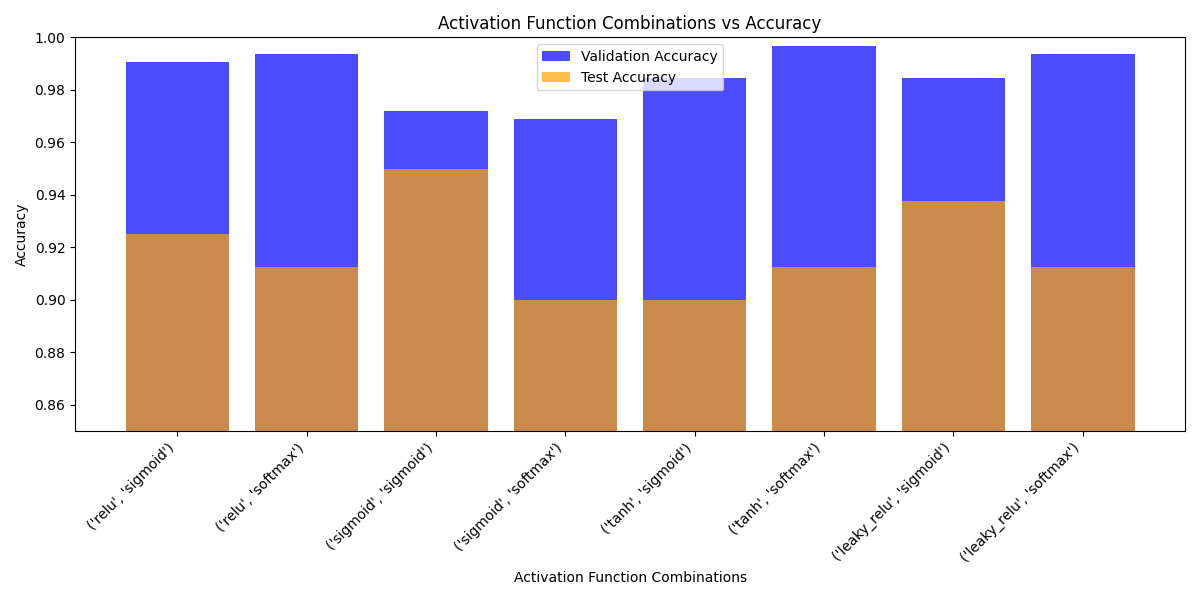
\includegraphics[width=0.5\textwidth]{images2/activation(2).png}
\centering
\caption{\label{fig:activation} Activation function vs  Accuracy}
\end{figure}
\par We can conclude that the best pair is (sigmoid,sigmoid), even though the validation accuracy is a little lower than the other pairs, the test data is really superior, showing greater capacity to predict data that was never used for train.
\paragraph{Results}
\par Now that the model is ready, It's time to show to results via the next figure 
\ref{fig:results_final}
and \ref{tab:nn_results}. The results are  good, however, the model is not perfect. The accuracy on test data is 95\%, which is apparently good, but if we observe the confusion matrix we can note that the model failed 4 predictions in 40 examples (2 examples per person), even not being bad, this model is behind many other machine learning algorithms.

\begin{figure}[H]
\hspace*{-1cm}
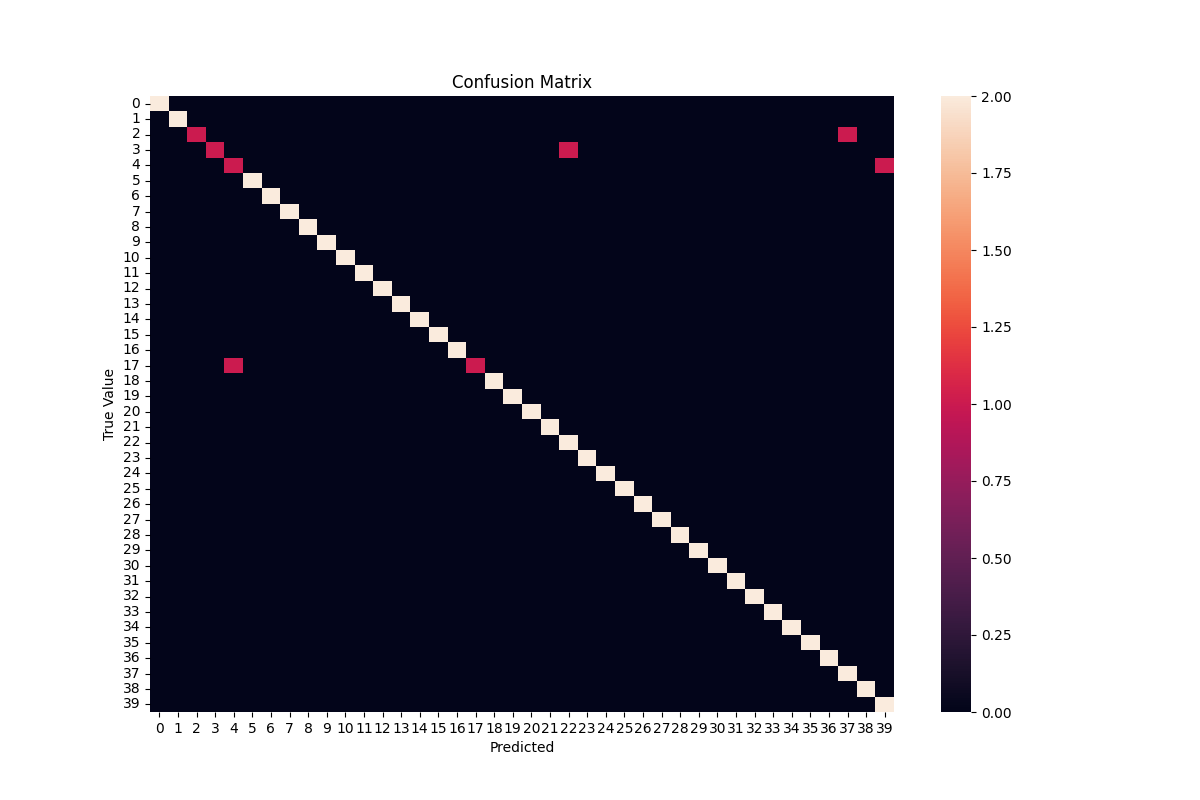
\includegraphics[width=0.6\textwidth]{images2/final_nn(1).png}

\caption{\label{fig:results_final} NN Confusion Matrix}
\end{figure}

\begin{table}[h!]
    \centering
\begin{tabular}{lrrr}
\toprule
{} &       accuracy  \\
\midrule
test  &  0.950 \\
train &  0.985  \\
val   &  0.991  \\
\bottomrule
\end{tabular}
    \caption{NN Results}
    \label{tab:nn_results}
\end{table}

\subsubsection{Logistic Regression}


\paragraph{Initial Configuration}
As we have already discussed, logistic regression is a crucial machine learning technique for facial recognition. In this section, we will go over the process of creating the logistic regression model. First, we had to confirm that our dataset contained no missing values. Next, we split the dataset into three subsets: 60\% for training data, 20\% for test data, and 20\% for validation data. This is necessary in order to assess the machine learning model.

\paragraph{Regularization}
First of all, solvers designed for larger datasets, like "saga" and "newton" may not perform as well as they could on the moderately sized Olivetti Dataset, which consists of 400 face images from 40 individuals. Their architecture, which is intended to handle larger datasets, may lead to less than ideal convergence and efficiency for this particular dataset.Moreover, the inclination towards L2 regularization in face recognition situations influences the selection of solvers such as "liblinear" and "lbfgs." These solvers better match the challenge of capturing complex facial patterns and fit in with the common regularization preferences in this field. Another thing to think about is convergence challenges, especially for the "saga" solver which can have problems with smaller datasets. Eliminating this solver reduces the possibility of reliability problems arising from convergence issues, guaranteeing a more stable. In summary, the exclusion of "saga" and "newton" solvers is a strategic decision based on the dataset's size, regularization preferences, convergence challenges, and considerations of computational efficiency in the specific context of face recognition.

\paragraph{Liblinear L1 Regularization}
Within the field of logistic regression for facial recognition, the L1 regularized "liblinear" solver is a particularly useful option. Because L1 regularization is known to induce sparsity in feature selection, it is a good fit for situations in which some facial features may contribute more than others. Given the moderate size of the Olivetti Dataset, the "liblinear" solver, which is optimized for small to medium-sized datasets, shows efficacy in our context. The model can concentrate on important facial features thanks to its effective handling of L1 regularization, which improves interpretability and may even improve generalization.
This is how we initially approached the logistic regression problem, and we analyze the outcomes below.

\begin{figure}[H]
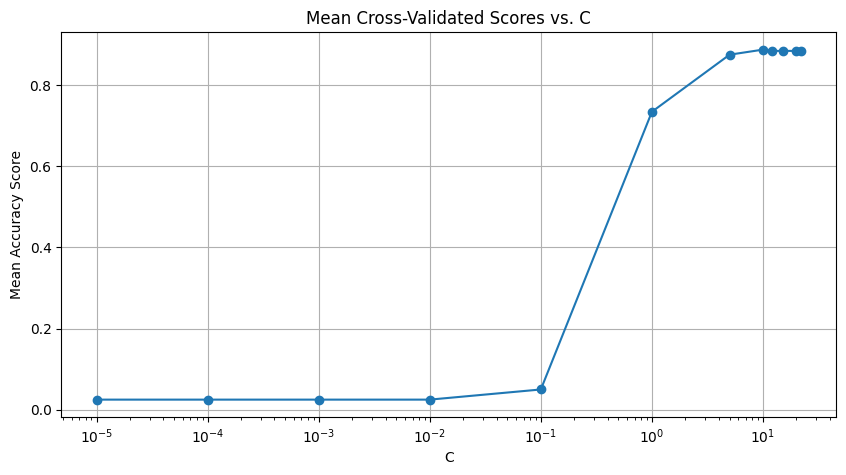
\includegraphics[width=0.5\textwidth]{images2/betterCL1.png}
\centering
\caption{\label{fig:CEvolL1} Mean Cross-Validated to find C}
\end{figure}

As can be seen in this graph\ref{fig:CEvolL1}, we can see that the best value of C is 20.
In scikit-learn's logistic regression implementation, the C parameter controls the strength of regularization applied to the model. Regularization is a technique used to prevent overfitting by adding a penalty term to the loss function, which discourages the model from fitting the training data too closely. The C parameter is the inverse of the regularization strength, meaning that smaller values of C result in stronger regularization, while larger values of C reduce the strength of regularization.

\begin{figure}[H]
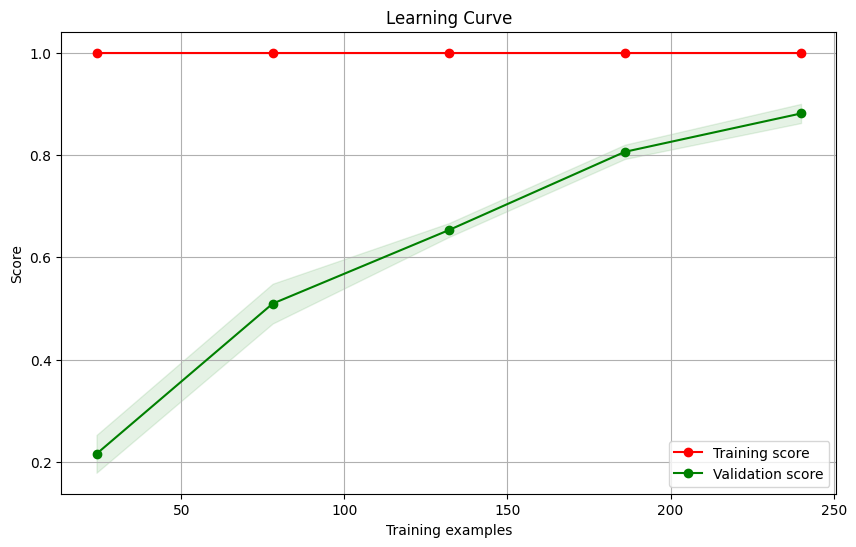
\includegraphics[width=0.5\textwidth]{images2/lcurveL1.png}
\centering
\caption{\label{fig:LCL1} Learning Curve for L1}
\end{figure}

On a learning curve\ref{fig:LCL1}, a significant difference between the validation and training scores suggests the possibility of overfitting. When a model overfits, it becomes too adapted to the training set and loses its ability to generalize well to new, untried data. This discrepancy indicates that the model might not function well in situations outside of the training set.

\begin{figure}[H]
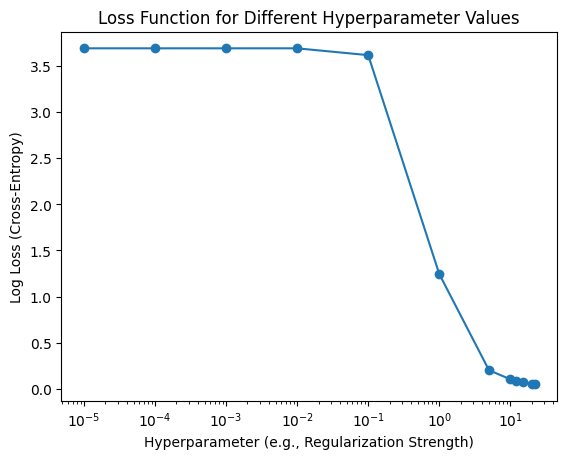
\includegraphics[width=0.5\textwidth]{images2/lossL1.png}
\centering
\caption{\label{fig:LossL1} Loss Function for L1 }
\end{figure}
The graph\ref{fig:LossL1} shows how different regularization strengths (hyperparameters) affect the logarithmic loss (cross-entropy), which is the loss function of the logistic regression model. A logarithmic scale with various hyperparameter values displayed on the x-axis illustrates the range of regularization strengths that have been tested. The corresponding log loss values are plotted on the y-axis to give an indication of how well the model predicts the training data while penalizing for complexity. Finding the regularization strength that strikes a balance between fitting the data and avoiding overfitting is the aim of the process. It involves minimizing the log loss. Reduced log loss values here signify better model performance.

For these hyperparameters the results are:
\begin{table}[h!]
    \centering
\begin{tabular}{lrrr}
\toprule
{}& Regularization &       Accuracy  \\
\midrule
train & L1 &  1.00  \\
test  & L1 &  0.9625 \\

\bottomrule
\end{tabular}
    \caption{L1 Regularization Results}
    \label{tab:resultsL1}
\end{table}




The outcomes\ref{tab:resultsL1} show that the logistic regression model with L1 regularization achieves a flawless 100\% on the training set, exhibiting remarkable accuracy. This shows that the model has picked up on the patterns in the training set of data successfully. With an accuracy of 96.25\% on the test set, the model maintains a strong performance, demonstrating its good generalization to new, untested data. All of these results point to the L1 regularization producing strong generalization performance across several datasets and successfully balancing model complexity to avoid overfitting.


\paragraph{Liblinear L2 Regularization}
Using the 'liblinear' solver with an L2 penalty in logistic regression turns out to be a dependable option when it comes to face recognition. This solver is effective for face recognition applications because it works well with small to medium-sized datasets. In order to encourage stable and well-behaved solutions, the L2 penalty, also referred to as Ridge regularization, adds the squared magnitude of coefficients to the model's cost function. A reliable and precise face recognition system is produced by combining the 'liblinear' solver with the L2 penalty, which strikes a balance between computational efficiency and model regularization.

\begin{figure}[H]
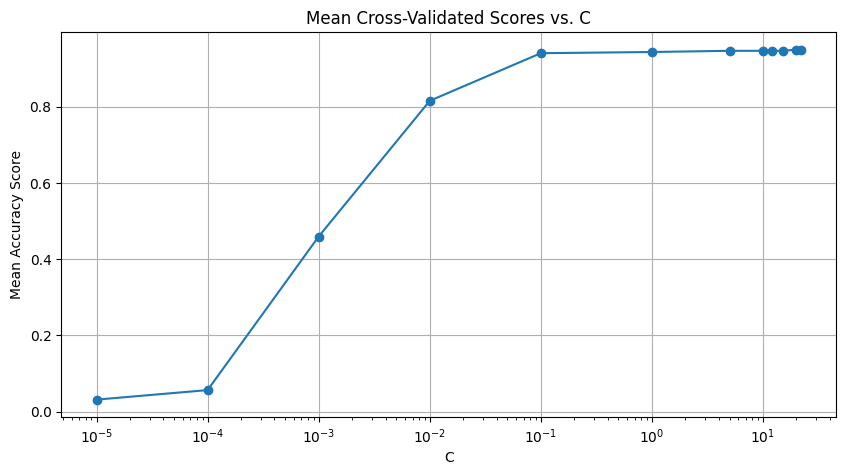
\includegraphics[width=0.5\textwidth]{images2/betteCL2.png}
\centering
\caption{\label{fig:CEvolL2} Mean Cross-Validated to find C }
\end{figure}
This graphic\ref{fig:CEvolL2} shows the mean cross-validated accuracy scores across various values of the regularization parameter (C) in logistic regression, as we discussed in the previous text. Given that it produces the highest mean accuracy score in this particular instance, C=20 looks to be the best regularization parameter. The regularization strength that maximizes the model's performance on unseen data has been successfully found by the grid search, highlighting the significance of fine-tuning hyperparameters for the best model results.



\begin{figure}[H]
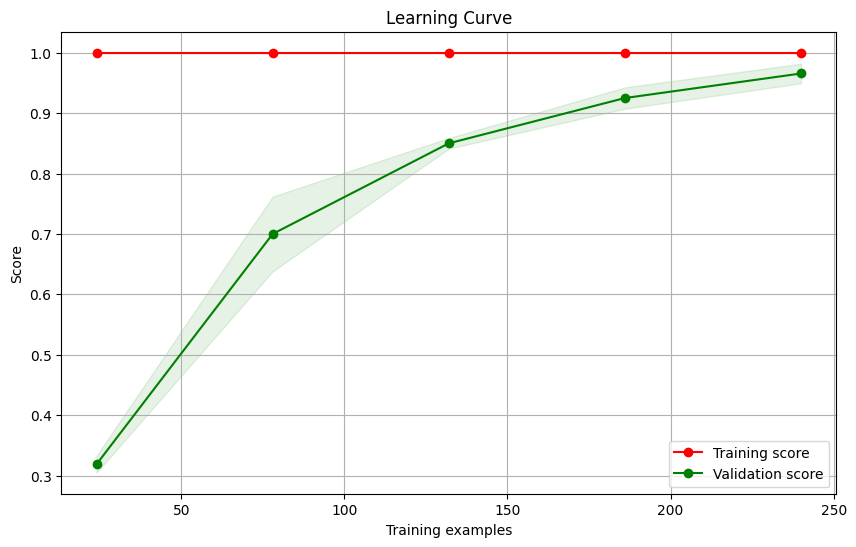
\includegraphics[width=0.5\textwidth]{images2/lcurveL2.png}
\centering
\caption{\label{fig:LCL2} Learning Curve for L2 }
\end{figure}

One improvement in the updated learning curve\ref{fig:LCL2} is the narrowing of the difference between the training and test scores. Improved convergence between the model's performance on the training set and its generalization to new, untested data is implied by this reduced space. This suggests a more balanced model with less overfitting tendencies and better ability to generalize learned patterns to different scenarios. A higher degree of robustness and good model adaptation to the training and validation datasets are indicated by the narrower separation, which shows a positive trajectory towards peak performance.

\begin{table}[h!]
    \centering
\begin{tabular}{lrrr}
\toprule
{}& Regularization &       Accuracy  \\
\midrule
train & L1 &  1.00  \\
test  & L1 &  0.9750 \\

\bottomrule
\end{tabular}
    \caption{L2 Regularization Results}
    \label{tab:resultsL2}
\end{table}



\paragraph{Results}
The results\ref{tab:resultsL2} show that using the Liblinear solver in conjunction with L2 regularization consistently produced better accuracy results than L1 regularization. The model that was trained using L2 regularization showed a perfect fit to the training data, achieving an astounding 100\% accuracy on the training set. Its strong accuracy scores of 97.50\% on the test set further demonstrated its superior generalization. This demonstrates how L2 regularization works better than L1 regularization in this situation, yielding a balanced model that performs well in training and unseen data scenarios.    

\begin{figure}[ht!]
\centering
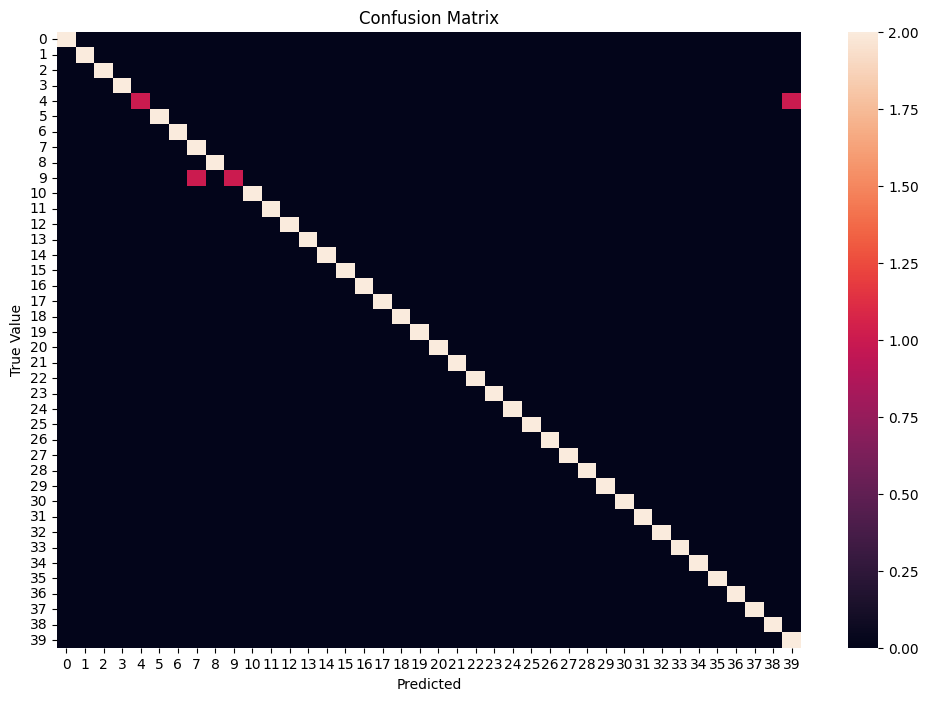
\includegraphics[width=0.5\textwidth]{images2/cmL2.png}

\caption{\label{fig:CML2} LR Confusion Matrix}
\end{figure}

Using either L1 or L2 regularization, our logistic regression model struggles to correctly identify the images linked to persons 4 and 9. As we can see in the confusion matrix\ref{fig:CML2}, the model seems to struggle particularly when faced with instances related to individuals bearing the identifiers 4 and 9, even though we have tried to fine-tune the hyperparameters using grid search and cross-validation.

\subsubsection{Support Vector Machine}


\paragraph{RBF Kernel}
A key component of Support Vector Machines (SVMs) is the RBF (Radial Basis Function) kernel, which is skilled at identifying complex patterns in data. For handling non-linear relationships, the RBF kernel excels by converting input features into a higher-dimensional space. Because SVMs can calculate the radial distance between data points, they are especially useful for capturing subtle patterns in a variety of datasets where boundaries are difficult to discern. Widely used in fields where non-linear relationships are common, like image recognition and bioinformatics, the RBF kernel is a flexible tool that is renowned for its adaptability. To put it simply, the RBF kernel helps support SVMs in navigating the complexity of different datasets, which helps machine learning models succeed in a variety of domains.
\begin{figure}[H]
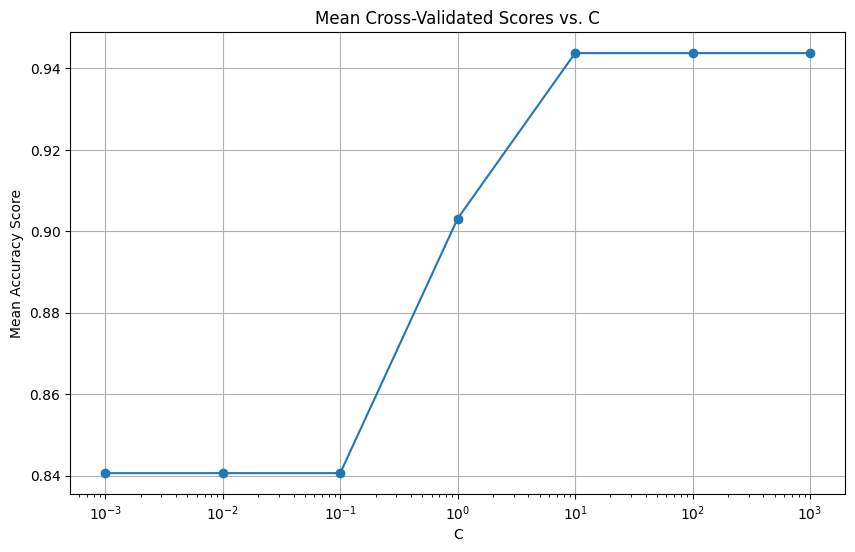
\includegraphics[width=0.5\textwidth]{images2/betterCRBF.png}
\centering
\caption{\label{fig:CEvolRBF} Mean Cross-Validated to find C}
\end{figure}
The mean accuracy scores illustrate the model's performance under various regularization settings as 'C' values rise on a logarithmic scale. The plot\ref{fig:CEvolRBF} prominently displays an ideal 'C' value of 10, it seams that the SVM reaches its maximum mean accuracy at this specific regularization strength. This realization is a useful reference for choosing the best hyperparameter when optimizing the SVM model for our approach.

\begin{figure}[H]
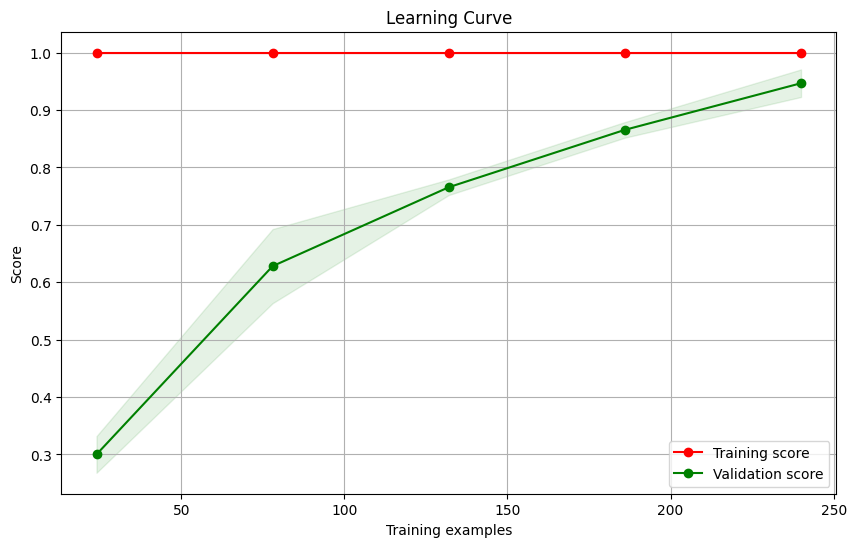
\includegraphics[width=0.5\textwidth]{images2/lcurveRBF.png}
\centering
\caption{\label{fig:LCRBF} Learning Curve for rbf kernel}
\end{figure}

The learning curve\ref{fig:LCRBF} demonstrates the model's capacity to identify intricate patterns in the data, with excellent training and validation set accuracies. Reasonable generalization appears to be indicated by the small difference between the training and test scores.

\begin{figure}[H]
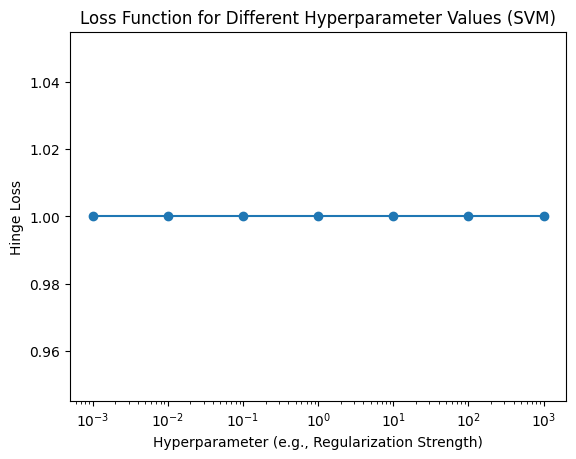
\includegraphics[width=0.5\textwidth]{images2/lossRBF.png}
\centering
\caption{\label{fig:LossRBF} Loss Function for rbf kernel}
\end{figure}

At y = 1.00, the hinge loss\ref{fig:LossRBF} is invariant to variations in the hyperparameter values. The loss function's stability shows that the SVM model regularly maintains a strong performance with little variation in classification errors when trained on the provided data.

\begin{table}[h!]
    \centering
\begin{tabular}{lrrr}
\toprule
{}& Kernel &       Accuracy  \\
\midrule
train & RBF &  1.00  \\
test  & RBF &  0.9750 \\

\bottomrule
\end{tabular}
    \caption{RBF Kernel Results}
    \label{tab:resultsRBF}
\end{table}



On the training set, the model attains perfect accuracy, demonstrating\ref{tab:resultsRBF} a deep comprehension of the underlying patterns in the data. The model's high test set accuracy (97.50\%) indicates that it can generalize well to new data. This is a good result, showing that the learned patterns of the model apply to fresh examples. In light of these findings, it's important to highlight that the model performs fairly well. 

\paragraph{Linear Kernel}
Since face recognition relies on identifying linear patterns and variations in facial features, the Linear Kernel's capacity to define distinct decision boundaries is particularly helpful in this domain. In situations where facial features are mainly linearly separable, the Linear Kernel works well, though it may not be able to capture very complex non-linear relationships.
Using the Olivetti dataset, the Linear Kernel in Support Vector Machines (SVMs) presents a simple and computationally effective method for face recognition, offering a dependable way to discern facial features along linear decision boundaries.

\begin{figure}[H]
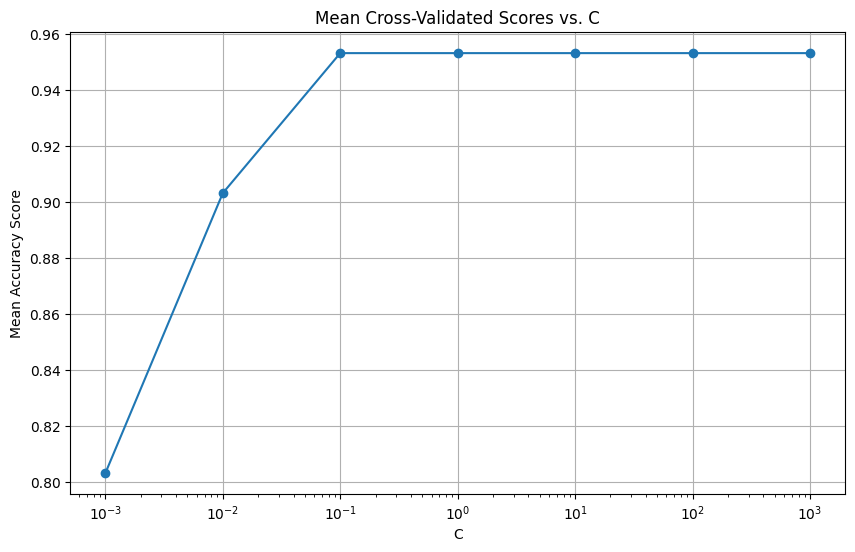
\includegraphics[width=0.5\textwidth]{images2/betterCLinear.png}
\centering
\caption{\label{fig:CEvolLi} Mean Cross-Validated to find C}
\end{figure}

From C = 0.1 onward, the graph\ref{fig:CEvolLi} shows a consistent trend in mean accuracy scores. This stability shows that the model's cross-validation performance, which measures its ability to generalize across a range of 'C' values, is consistently high. The study of various regularization strengths is presented on the x-axis logarithmic scale, and the stability that is observed is a useful indication of how well the model maintains its accuracy, especially when C = 0.1 and higher.

\begin{figure}[H]
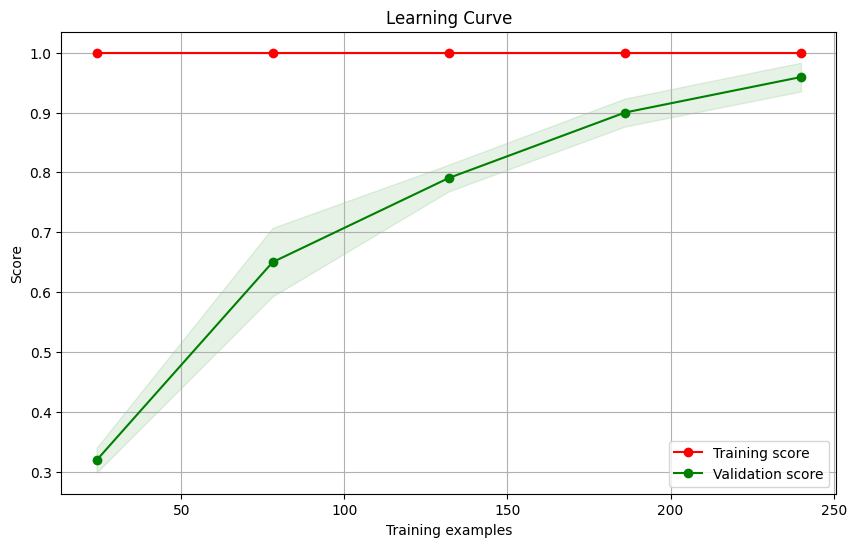
\includegraphics[width=0.5\textwidth]{images2/lcurveLinear.png}
\centering
\caption{\label{fig:LCLi} Learning Curve - Linear Kernel}
\end{figure}

The linear kernel's updated learning curve graph\ref{fig:LCLi} confirms the earlier noted positive trajectory. The model shows great learning capabilities and achieves almost perfect accuracy on the training set. This iteration's improved test score, which highlights the model's improved generalization to untested data, is noteworthy. We found in our SVM analysis that the model's accuracy on the test data was not significantly affected by the choice between linear kernels and RBF. 

\begin{figure}[H]
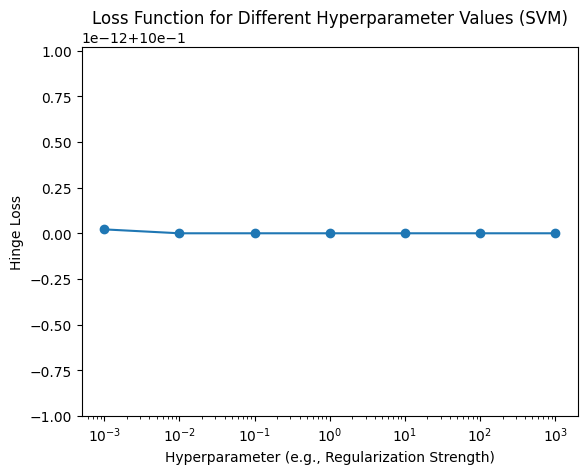
\includegraphics[width=0.5\textwidth]{images2/lossLinear.png}
\centering
\caption{\label{fig:LossLi} Loss Function - Linear Kernel}
\end{figure}

On the other hand, a consistent value is observed\ref{fig:LossLi} along the y-axis in the hinge loss plot of the SVM model with a linear kernel. However, this value is centered around y = 0, in contrast to the RBF kernel, which revealed a constant hinge loss at y = 1.00, the linear kernel's stability at y = 0 suggests a stable margin and class separation. This implies that the linear kernel accomplishes this by successfully keeping the decision values well within the margin, all the while maintaining a uniform loss.

\paragraph{Results}


\begin{table}[h!]
    \centering
\begin{tabular}{lrrr}
\toprule
{}& Kernel &       Accuracy  \\
\midrule
train & RBF &  1.00  \\
test  & RBF &  0.9750 \\

\bottomrule
\end{tabular}
    \caption{Linear Kernel Results}
    \label{tab:resultsLi}
\end{table}


With a perfect accuracy of 100.00\% on the training set, the SVM demonstrates its capacity to accurately learn from the given data. In addition, the model achieves a high accuracy of 97.75\% on the test set, demonstrating robust generalization to unknown examples. These outcomes\ref{tab:resultsLi} highlight the SVM's ability to accurately predict both seen and unseen data, as well as its efficacy in identifying complex patterns within facial images.


\begin{figure}[ht!]
\centering
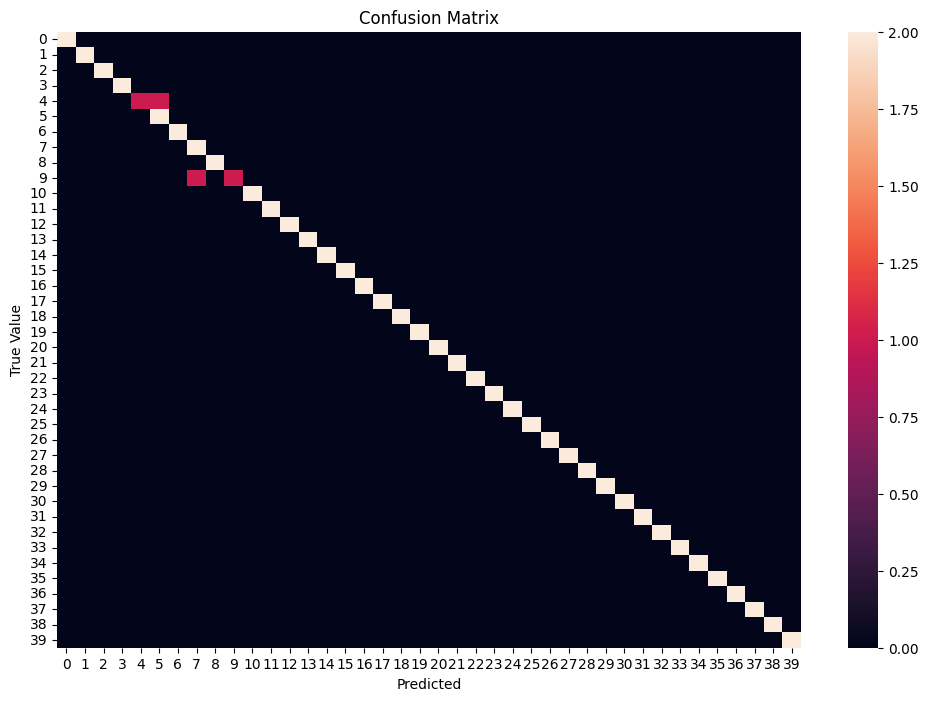
\includegraphics[width=0.5\textwidth]{images2/cmLinear.png}

\caption{\label{fig:CMLi} SVM Confusion Matrix}
\end{figure}

In our SVM model, the linear and RBF kernels use different kernels, but their accuracy rates are the same. Interestingly, the confusion matrix shows\ref{fig:CMLi} that both kernels face difficulties in correctly identifying the faces connected to persons 4 and 9. This mutual constraint implies that the problem extends beyond the selection of the kernel and calls for additional research into possible data-specific subtleties influencing the model's capacity to identify these specific users. 

\section{Comparison between the models}
\subsection{Comparison with average results on Olivetti Dataset}
We are preparing to perform a thorough comparison with the Olivetti Faces dataset as part of our ongoing effort to assess and benchmark the performance of our models. This comparative study\ref{fig:resultC} will help us comprehend our models' advantages and shortcomings in the larger context of facial image classification.
\begin{figure}[H]
\centering
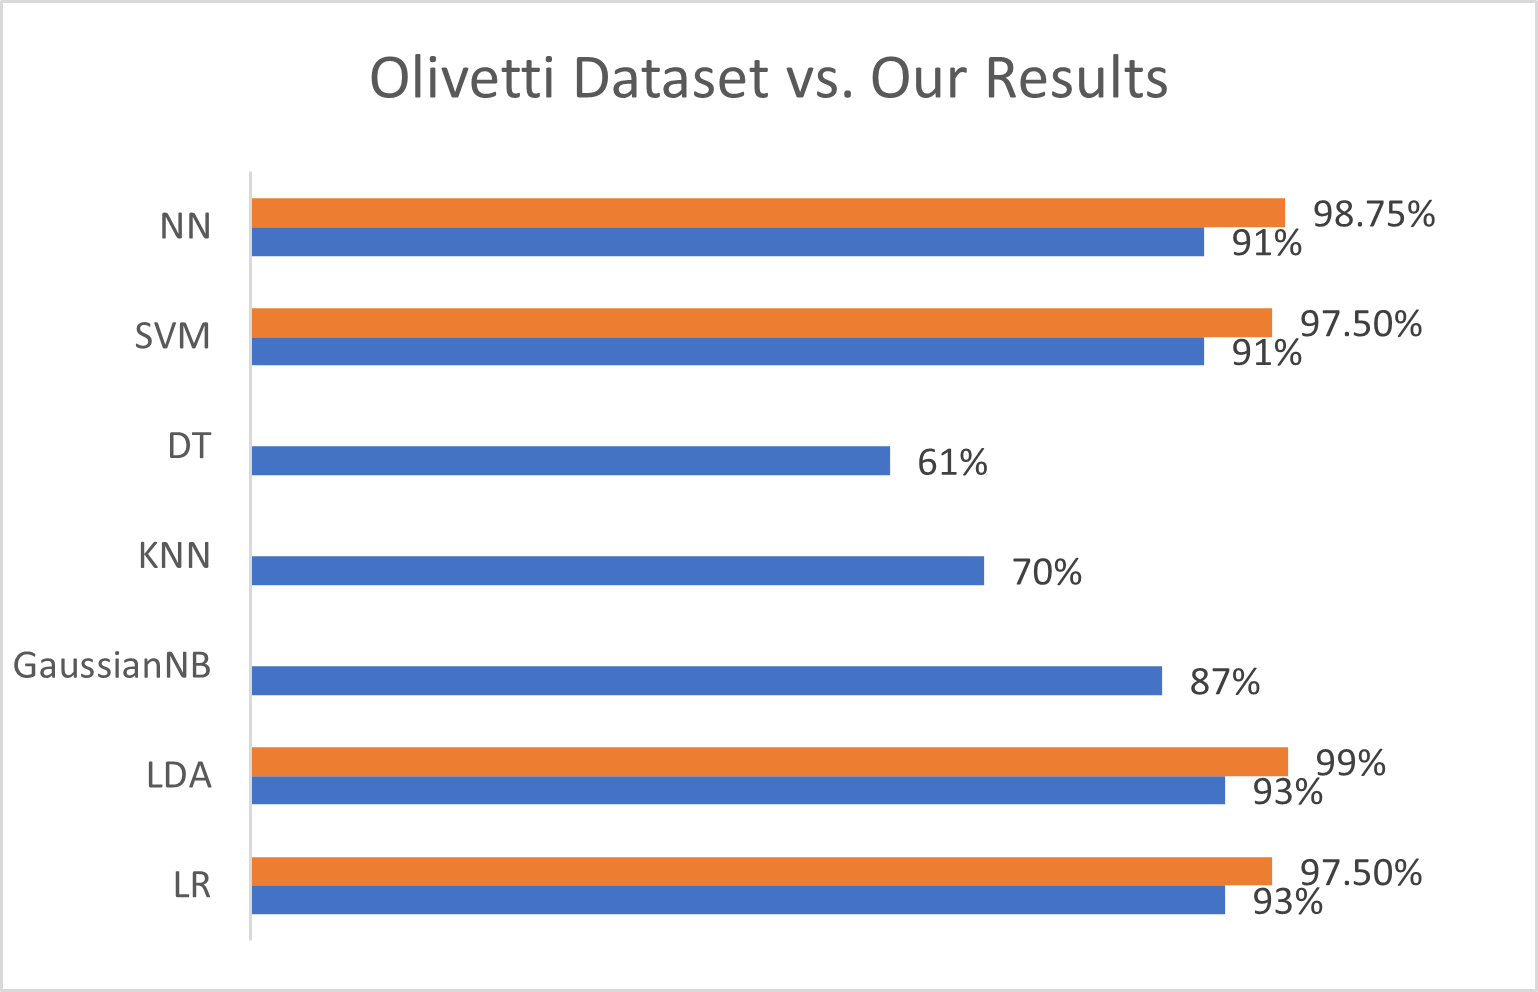
\includegraphics[width=0.5\textwidth]{images2/results.png}

\caption{\label{fig:resultC} Results from other works on Olivetti Dataset vs Our Results}
\end{figure}



With a 97.75\% accuracy rate, our SVM model demonstrates its remarkable predictive precision. Despite the SVM's commendable 91\% accuracy rate, our method may be better at identifying the underlying patterns in the data based on the difference in accuracy between the two models.
The mean results of other works achieves 93\% accuracy in logistic regression, our model performs better, having  97,50\% accuracy.
Our LDA model performs with  99 \% accuracy, being this value considerably higher comparing with the one in the figure with 93\%.
Finally, the ANN  we developed  demonstrates a good performance having 95\% accuracy which is above average as well, being that value usually around  91\%.
\subsection{Comparison between our models}
\par As we discussed before, we have a really good tool to compare models which is ROC curve \ref{fig:roc}. The Roc curve will evaluate our model based on True positive vs False positive,i.e., what is the ratio between number of times we predicted a face correctly vs a wrong prediction.The bigger the area under the curve is better is the performance of the model. It's possible to see that all models except NN have similar performances, having all area equal to 1, meaning perfect performance, however this values are rounded, so, by observing the figure it's possible to get more details, concluding so that LDA has the bigger are, then LR and finally SVM. NN has a good AUC, however is bellow the other models.

\begin{figure}[H]
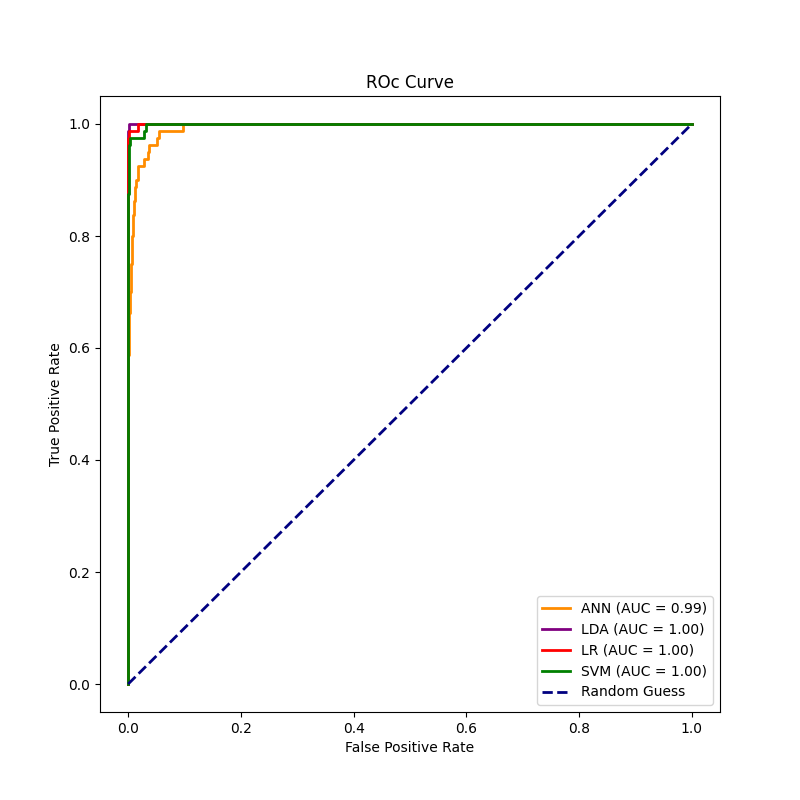
\includegraphics[width=0.5\textwidth]{images2/ROC.png}
\centering
\caption{\label{fig:roc} Roc Curve}
\end{figure}

\par One thing we noted is that every model failed predicting specific face, which  face id 4, more specificly, this picture \ref{fig:id4}, however we didn't conclude Why it happen since the picture doesn't goes out of the pattern compared with other picture of the same person.\ref{fig:id4_2}

\begin{figure}[H]
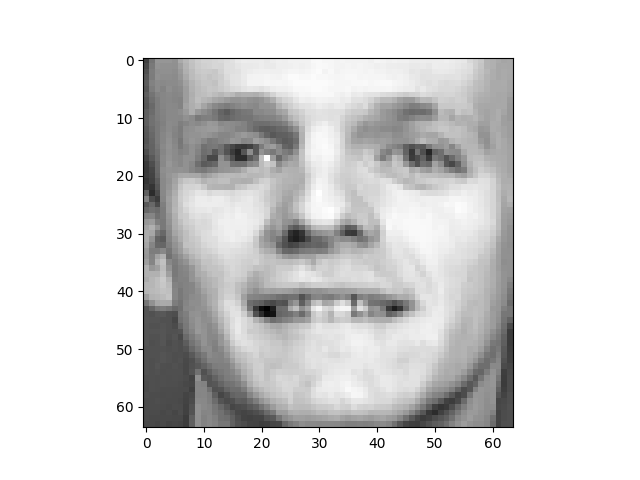
\includegraphics[width=0.1\textwidth]{images2/id4.png}
\centering
\caption{\label{fig:id4} Face id 4}
\end{figure}

\begin{figure}[H]
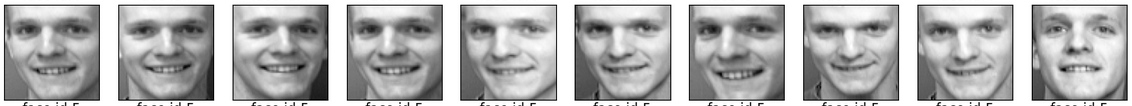
\includegraphics[width=0.4\textwidth]{images2/id4_2.PNG}
\centering
\caption{\label{fig:id4_2} Faces of id 4}
\end{figure}

\subsection{Comparison with state of the art works}
\begin{itemize}
    \item Face Recognition System Using Machine Learning Algorithm \cite{state1} - This work reached a 100\% accuracy with one specific configuration using the same dataset as us. The explanation of this paper getting better results, probably comes from an utilization of different configurations. Those configurations consist on  changing the size of the training data and testing data in each of them. Analogous to our work, they tried different machine learning algorithms.
    \item Gabor Filter-Based Face Recognition Technique\cite{state2} - This paper presents an accuracy of 90\%. It highly focus on data pre-processing, which is an important step in computer vision and is a point that we should had explore more exhaustively during our work. These results were worse than ours, because the data-set was different, so it's impossible to compare directly with us, besides that, the paper refers a high performance of the model when detecting frontal faces, which is similar case with our dataset, so we assume a bigger accuracy of the paper.
    \item  Face Recognition with Very Deep Neural Networks \cite{state3} - This work achieved great results, reaching 99.53\% accuracy, a result that is even higher than our best model, furthermore, the dataset used in this work present faces with different angles,i.e, not only front pictures, so the results are even more impressive. This model reach a better performance classifying, because they used a really complex model with many, many layers of feature extraction, that's why it's called very deep neural network. An architecture like that has lot more prediction capability , due to a much bigger level of complexity compared to our work, that is relatively simple.
\end{itemize}



\section{Conclusion}
To sum up, our experience with machine learning for facial recognition has been rewarding. We have committed to improving our knowledge of different algorithms throughout this project, with an emphasis on Support Vector Machines, Linear Discriminant Analysis, Logistic Regression, and Neural Networks. Combining these various methods has strengthened our strategy and given us a more comprehensive and nuanced view of the complexities and difficulties involved in facial recognition.




\section{Contributions}
In this project we tried to divide the work equally, João created and trained the Linear Discriminant Analysis and Neural Network models and Guilherme the Logistic Regression and Support Vector Machine model. At a later stage, writing the report was also divided equally.

\begin{table}[h!]
    %\centering
\begin{tabular}{lrrr}
\toprule
{} &       Contributions \\
\midrule
João Rodrigues	& 50\% \\
Guilherme Casal & 50\% \\
\bottomrule
\end{tabular}
    
\end{table}


\nocite{Paper5,Paper1,Paper3,sklearn,mastromichalakis2021alrelu,misc_breast_cancer,Paper4,tensorflow,roc} 
\printbibliography

%\cite{misc_breast_cancer} and this %\cite{Smith:2013jd}.


% See this guide for more information on BibTeX:
% http://libguides.mit.edu/content.php?pid=55482&sid=406343

% For more author guidance please see:
% http://wellcomeopenresearch.org/for-authors/article-guidelines

% When all authors are happy with the paper, use the 
% ‘Submit to WELLCOME OPEN RESEARCH' button from the menu above
% to submit directly to the open life science journal Wellcome Open Research.

% Please note that this template results in a draft pre-submission PDF document.
% Articles will be professionally typeset when accepted for publication.

% We hope you find the Wellcome Open Research Overleaf template useful,
% please let us know if you have any feedback using the help menu above.



\end{document}